\chapter{Enclosure and Mount Design}
\label{app:mechanical}

This appendix records the mechanical design of the printed assemblies that put the system on the vehicle: the dashboard display mount, the two sensor pods (rear for the Raspberry Pi~4 and the telemetry unit, front for the Raspberry Pi~5), and the two IMU pods. It gives the measurements each design rests on, the choices made and why, the checks run on the three-dimensional geometry, and the print plan. All were modelled in SOLIDWORKS 2025, or edited as meshes, and sliced for the Prusa MINI. On 12 October none had been printed; the pods were printed and mounted on the vehicle for the road session of 19 October, and the display mount is being redesigned. The checks below are on the CAD geometry, not on physical parts.

The parts were built by Python scripts that drive SOLIDWORKS through its API (\texttt{CAD/*/build/} in the repository). Every size comes from one parameter list, so a new measurement is one number and a rebuild. The scripts are the source of truth: most sketches are not dimensioned inside SOLIDWORKS, so editing a dimension in SOLIDWORKS does not drive the model.

\section{Requirements and measurements}
\label{sec:mech-requirements}

Table~\ref{tab:mech-inputs} lists the inputs. Where a value was measured it was used; where it was not, it is marked as an estimate and listed in Section~\ref{sec:mech-outstanding}. Figure~\ref{fig:mech-measurements} shows two of the measurement records.

\begin{table}[htbp]
\centering
\caption{Inputs to the enclosure and mount designs.}
\label{tab:mech-inputs}
\small
\begin{tabular}{|p{4.6cm}|p{3.4cm}|p{6.4cm}|}
\hline
\textbf{Item} & \textbf{Value} & \textbf{Source} \\ \hline
Display outline (Waveshare 10.1\,in HDMI LCD (B) in its case) & 272 by 187\,mm & Measured; the manufacturer's drawing gives 274.12\,mm, so the long side is to be confirmed \\ \hline
Display depth & 20\,mm & Estimate; the manufacturer gives 18\,mm without a computer behind it \\ \hline
Display connector span & 43 to 45\,mm & Measured \\ \hline
Space at the vehicle's meter & about 305\,mm across & Tape photograph, 2 September \\ \hline
Handlebar diameter & 22.2\,mm & Standard 7/8\,in bar; not yet measured on the vehicle \\ \hline
Raspberry Pi~4 and~5 & 85 by 56\,mm, M2.5 holes on 58 by 49\,mm & Official mechanical drawings \\ \hline
ESP32-S3 A7670X board & 75 by 52\,mm, M2 holes on 71 by 48\,mm & Manufacturer's board file (V1.2; the fitted board is V1.1) \\ \hline
ToF sensor board outline & 86, 41, 22 and 30\,mm edges; 14\,mm above and 6\,mm below the PCB & Measured; mounting holes estimated from a photograph \\ \hline
Camera in its printed case & 29.2 by 28.2 by 12.35\,mm & Measured from its STL \\ \hline
ToF field of view & 25$^\circ$ cone & Datasheet \\ \hline
Camera field of view & 53.5 by 41.4$^\circ$ & Raspberry Pi documentation \\ \hline
Printer & Prusa MINI, 180 by 180 by 180\,mm & Available printers \\ \hline
GY-521 IMU board & 20 by 17\,mm & Measured; hole spacing 15.2\,mm to be measured \\ \hline
\end{tabular}
\end{table}

\begin{figure}[htbp]
\centering
\subfigure[Display, Raspberry Pi~5 and IMU sizes recorded on the whiteboard.]{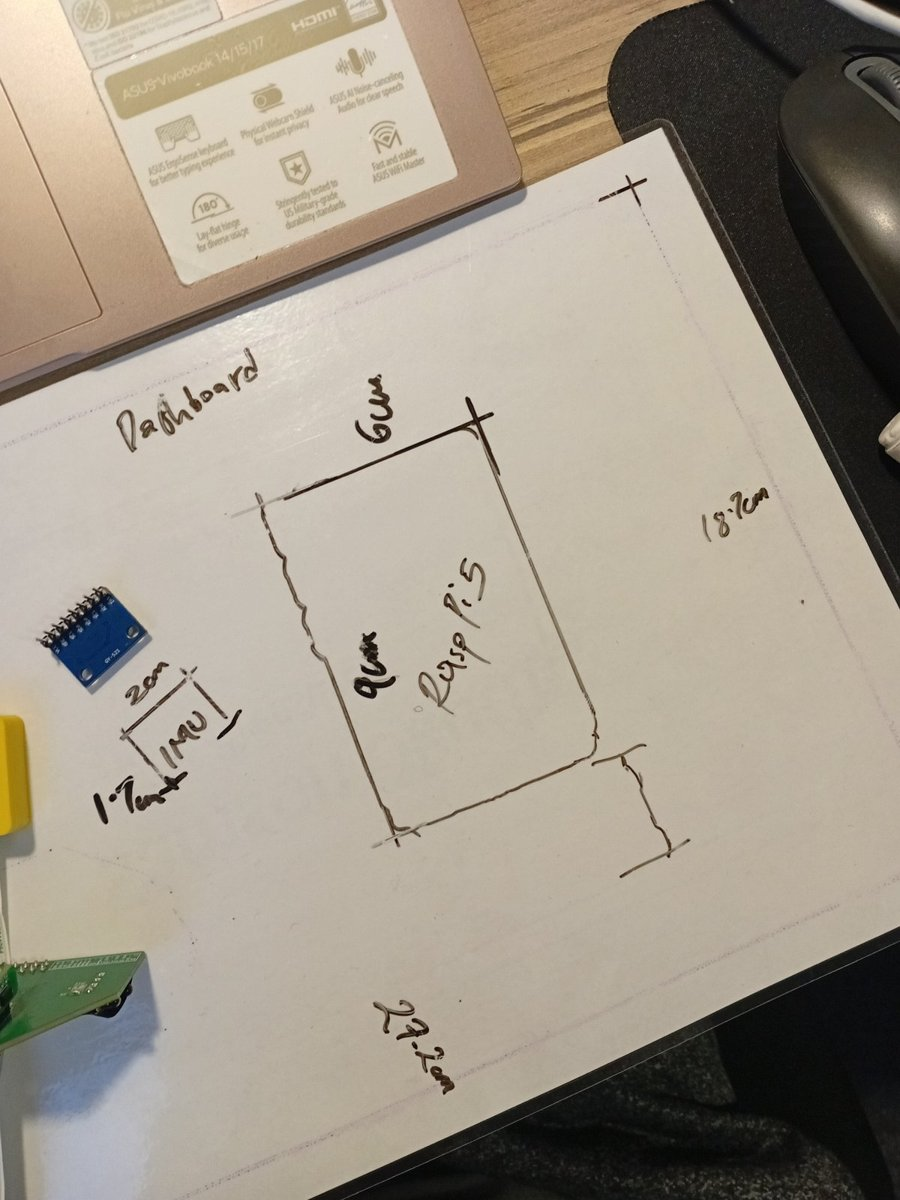
\includegraphics[width=0.38\textwidth]{figures/cad/photo_whiteboard_sizes.jpg}}
\hspace{0.03\textwidth}
\subfigure[The camera in its case above the ToF sensor board, joined by the ribbon, in the layout the pod keeps.]{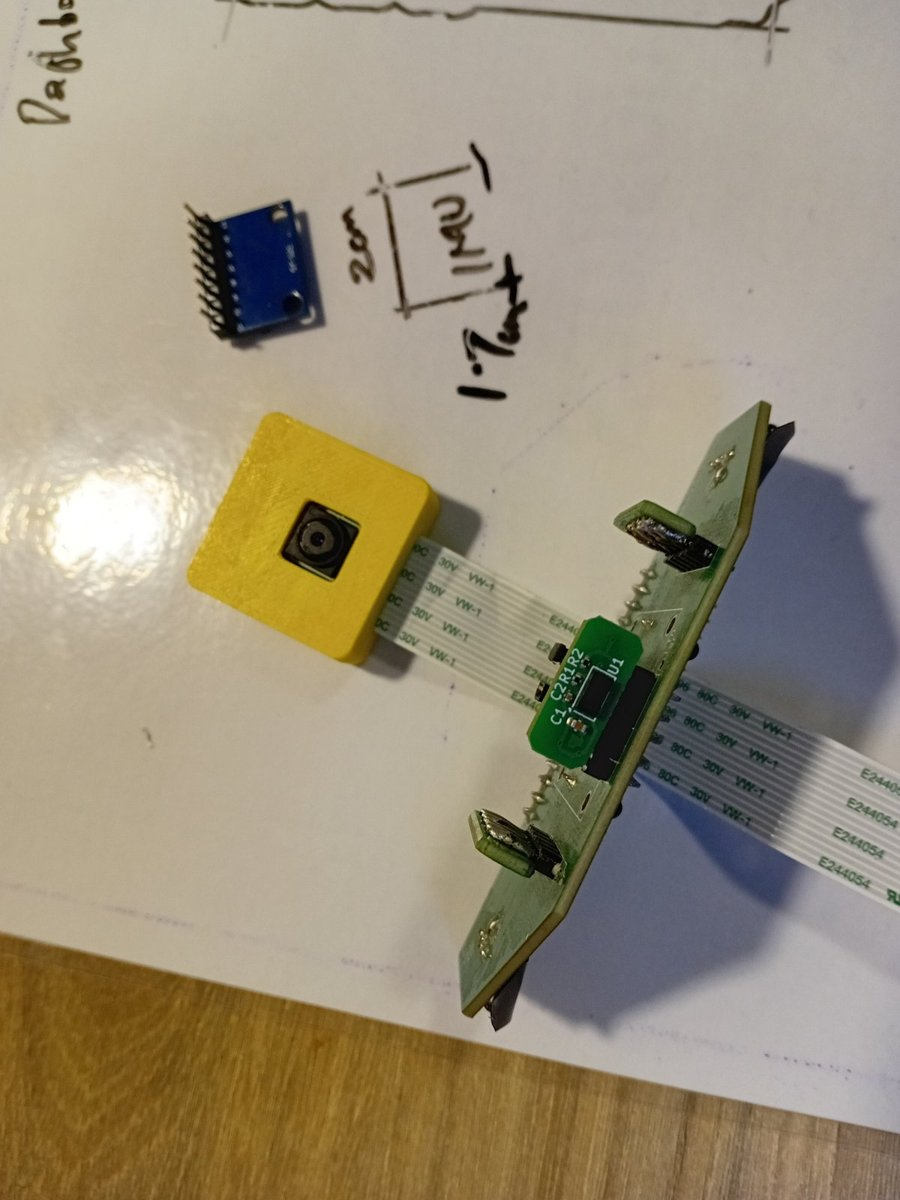
\includegraphics[width=0.38\textwidth]{figures/cad/photo_board_and_camera.jpg}}
\caption{Measurement records for the enclosure designs.}
\label{fig:mech-measurements}
\end{figure}

\section{Design choices}
\label{sec:mech-choices}

Table~\ref{tab:mech-choices} gives each main choice, the alternatives considered and the reason. The deciding constraints were the 180\,mm print bed, the need to remove the electronics from the vehicle without tools, the sensors' fields of view, and sun and rain.

\begin{table}[htbp]
\centering
\caption{Main design choices for the enclosures and mounts.}
\label{tab:mech-choices}
\small
\begin{tabular}{|p{3.4cm}|p{3.6cm}|p{7.4cm}|}
\hline
\textbf{Choice} & \textbf{Alternatives} & \textbf{Reason} \\ \hline
Bar clamp with a dovetail rail and a locking thumb screw & Adhesive pads, straps, a fixed screw mount & The display and pod come off without tools for charging, security and work on the bench. The channel's closed end carries the weight. The thumb screw drops into a detent in the rail, so the part cannot lift out over bumps. One clamp design serves both the display and the pod \\ \hline
Display above the handlebar, like a phone mount & Display centred on the bar & With the bar behind the display's centre, half the display would hang towards the driver's knees. Above the bar it stays in the line of sight at the meter \\ \hline
Display shell printed in four quarters joined by bolted plates & One piece on a larger printer & The shell is 278 by 193\,mm, larger than the 180\,mm bed in both directions. The plates carry load: the rail plate and the Pi~5 cradle are also joints \\ \hline
Raspberry Pi~5 on a cradle outside the shell & Inside the shell & Inside, the shell would grow from 27 to about 45\,mm deep. Outside, the Pi has air for its cooler, and its cables to the display's connector side stay short \\ \hline
Cable exit as an open notch on the connector side & A closed window & It matches the 43 to 45\,mm connector span, and it has no roof to print over the plugs \\ \hline
Sensor pod as a head and a box bolted together & One housing; a separate remote box & One housing exceeds the bed. A remote box would exceed the camera's 15\,cm ribbon (the ribbon path is about 115\,mm). The box also keeps the Pi's heat and the GNSS antenna away from the sensors \\ \hline
Open, flared ToF windows with drip hoods & A window covering the sensors & VL53L0X ranging degrades behind most plastics. The window flares 5$^\circ$ wider than the 25$^\circ$ cone, and a hood keeps rain off \\ \hline
Camera centred above the sensor board & Camera beside the board & This keeps the student's layout. Camera and ahead sensor share a centre line, and the cones show the camera's view clear of the ToF windows \\ \hline
GNSS patch under a 1.2\,mm plastic roof & An external antenna & No metal or carbon-filled filament above the patch. One cable fewer \\ \hline
Heat-set inserts for every repeated joint & Screws into printed plastic & The joints survive being opened many times \\ \hline
Faceted outer form with a light-bar groove & A plain box & It follows the TUKZIE concept renders without costing function \\ \hline
IMU pods on the handlebar stem and the rear chassis, keyed by an arrow & One pod; loose boards & These are the positions in the vehicle integration and test plan (SW7-VIT-001), which follows the vacation-work teams' layout. The arrow fixes each board's axes relative to the vehicle \\ \hline
\end{tabular}
\end{table}

\section{Dashboard display mount}
\label{sec:mech-dashboard}

Figure~\ref{fig:mech-dash-assembly} shows the assembly on a dummy 22.2\,mm bar, with stand-in bodies for the display and the Raspberry Pi~5. The model frame is face down: the screen faces up in the pictures. Figure~\ref{fig:mech-dash-parts} shows the printed parts, and Table~\ref{tab:mech-dash-parts} lists them. To fit the display, the clamp is bolted round the bar over a 1\,mm rubber strip and turned to set the screen's tilt. The display slides down onto it, and the thumb screw is turned up into the detent.

\begin{figure}[htbp]
\centering
\subfigure[Isometric view.]{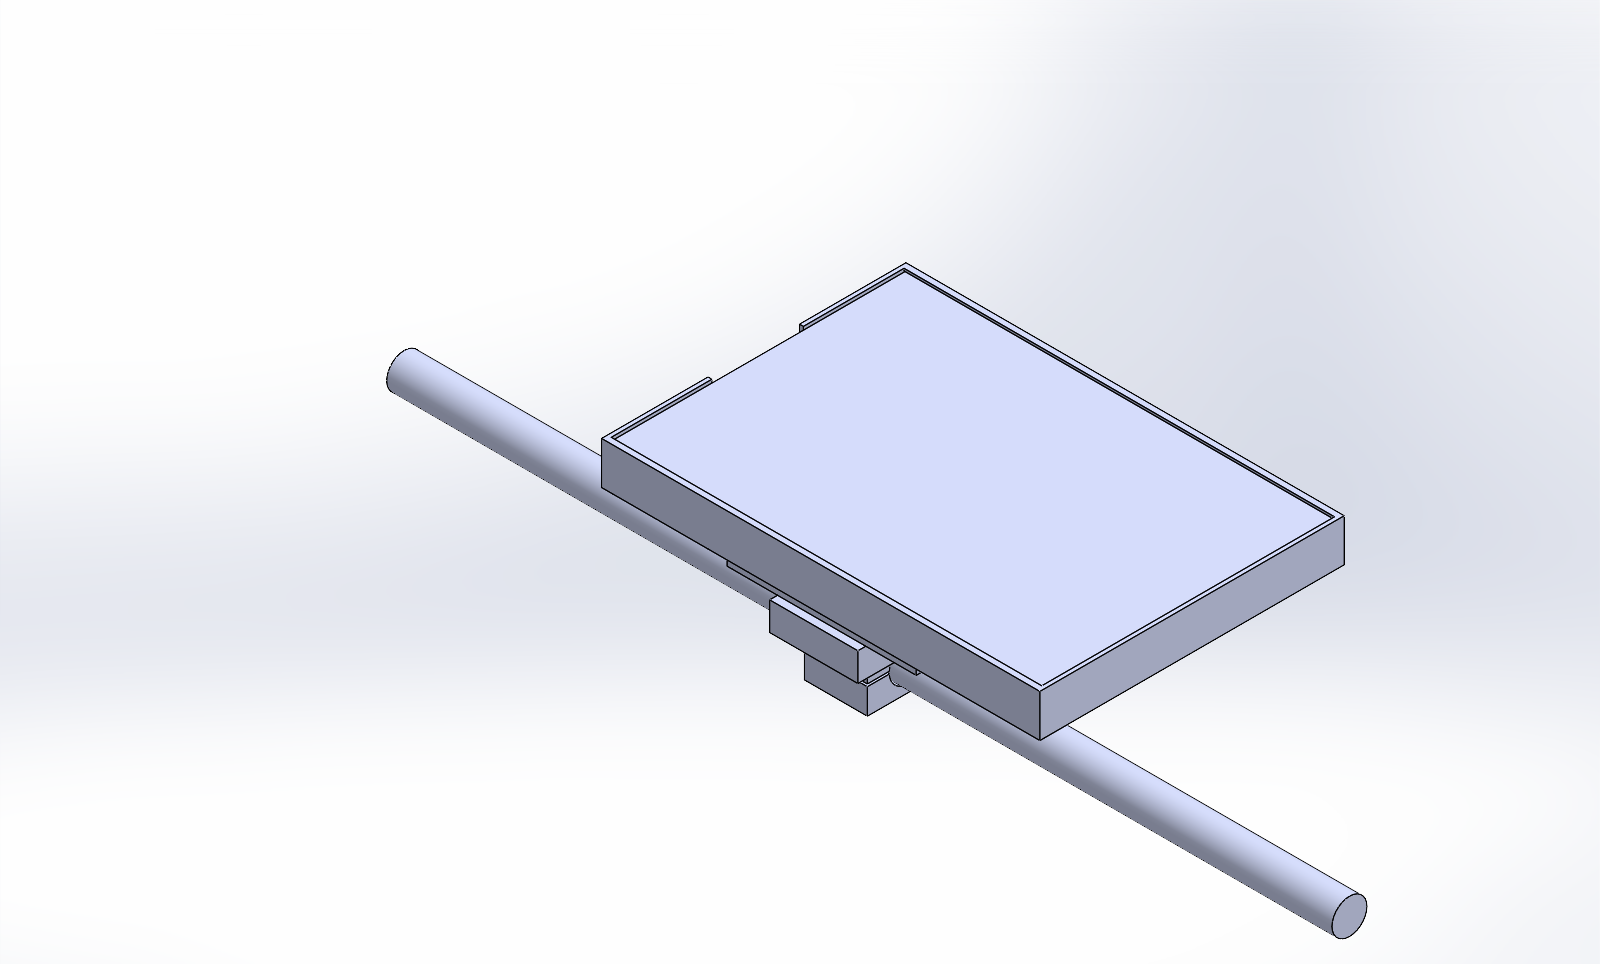
\includegraphics[width=0.48\textwidth]{figures/cad/dash_assembly_iso.png}}
\subfigure[From behind: rail plate, Pi~5 cradle, joiner plates and clamp.]{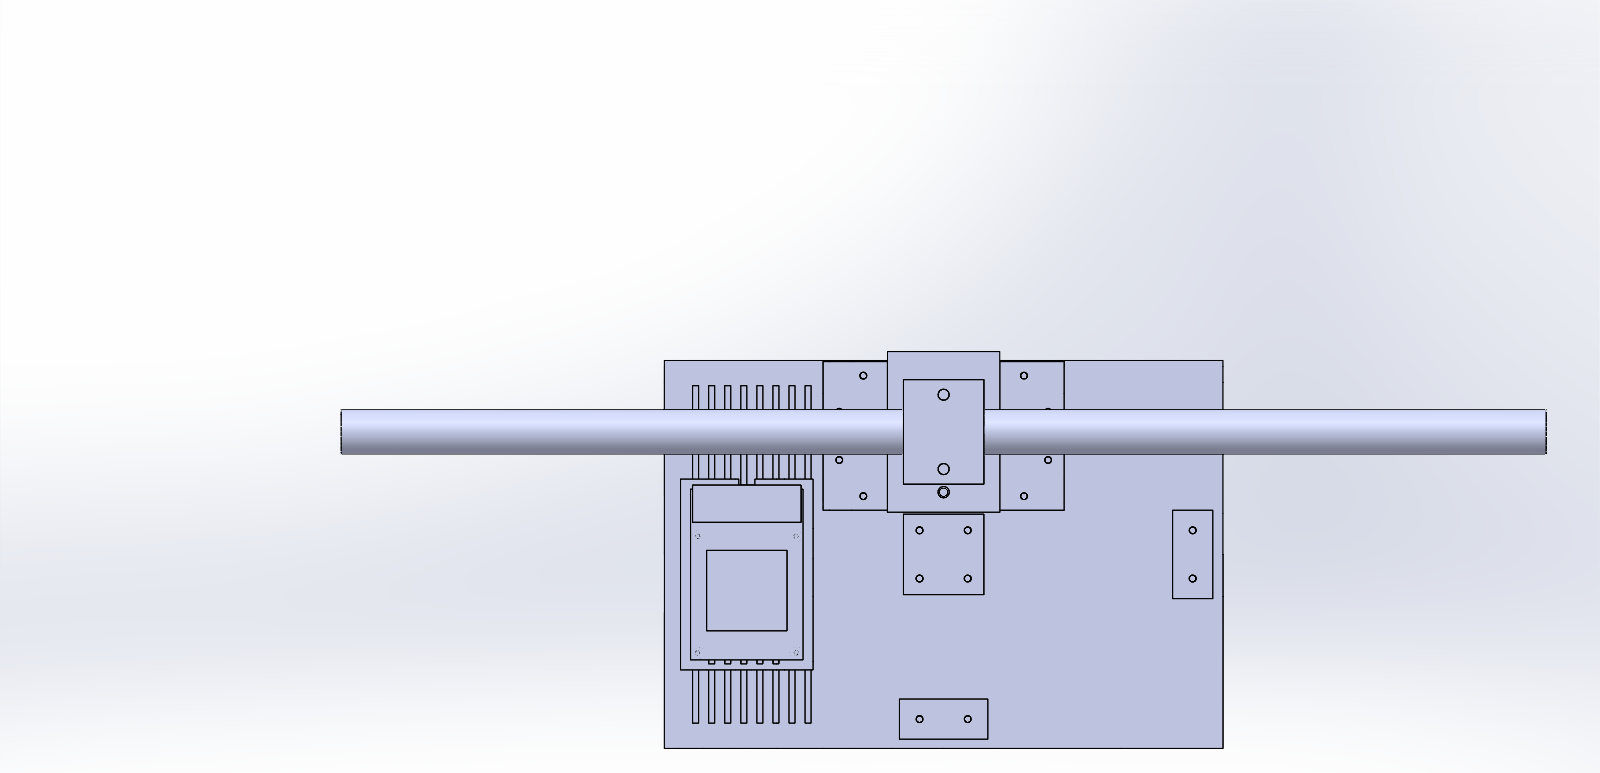
\includegraphics[width=0.48\textwidth]{figures/cad/dash_assembly_back.png}}
\subfigure[Side view: shell, rail plate, bracket, clamp cap and bar.]{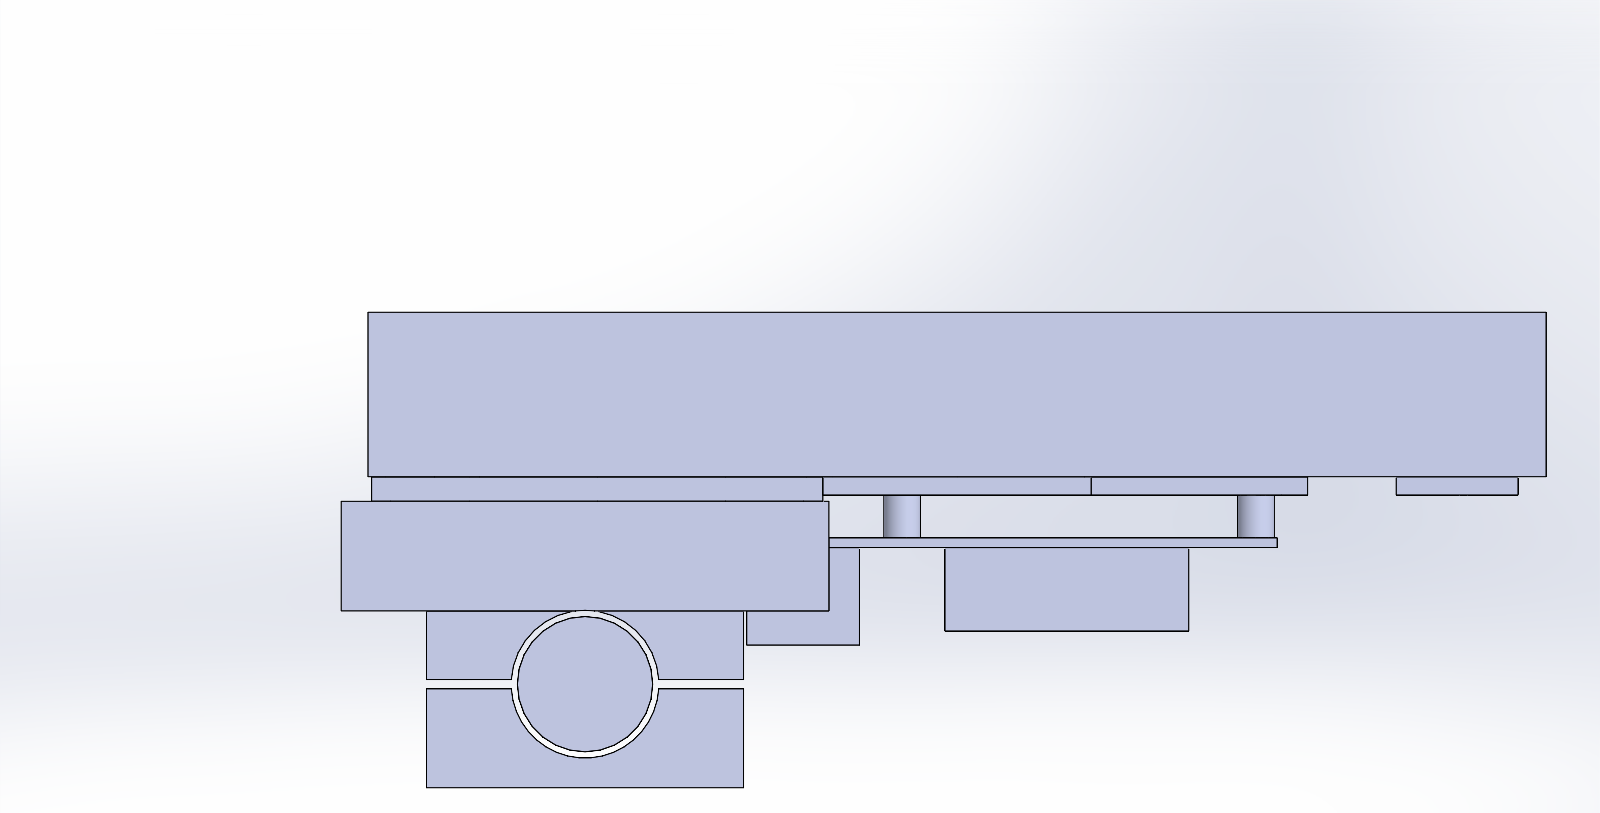
\includegraphics[width=0.7\textwidth]{figures/cad/dash_assembly_side.png}}
\caption{Dashboard display mount assembly (revision 2).}
\label{fig:mech-dash-assembly}
\end{figure}

\begin{figure}[htbp]
\centering
\subfigure[Bracket: dovetail channel and upper clamp half.]{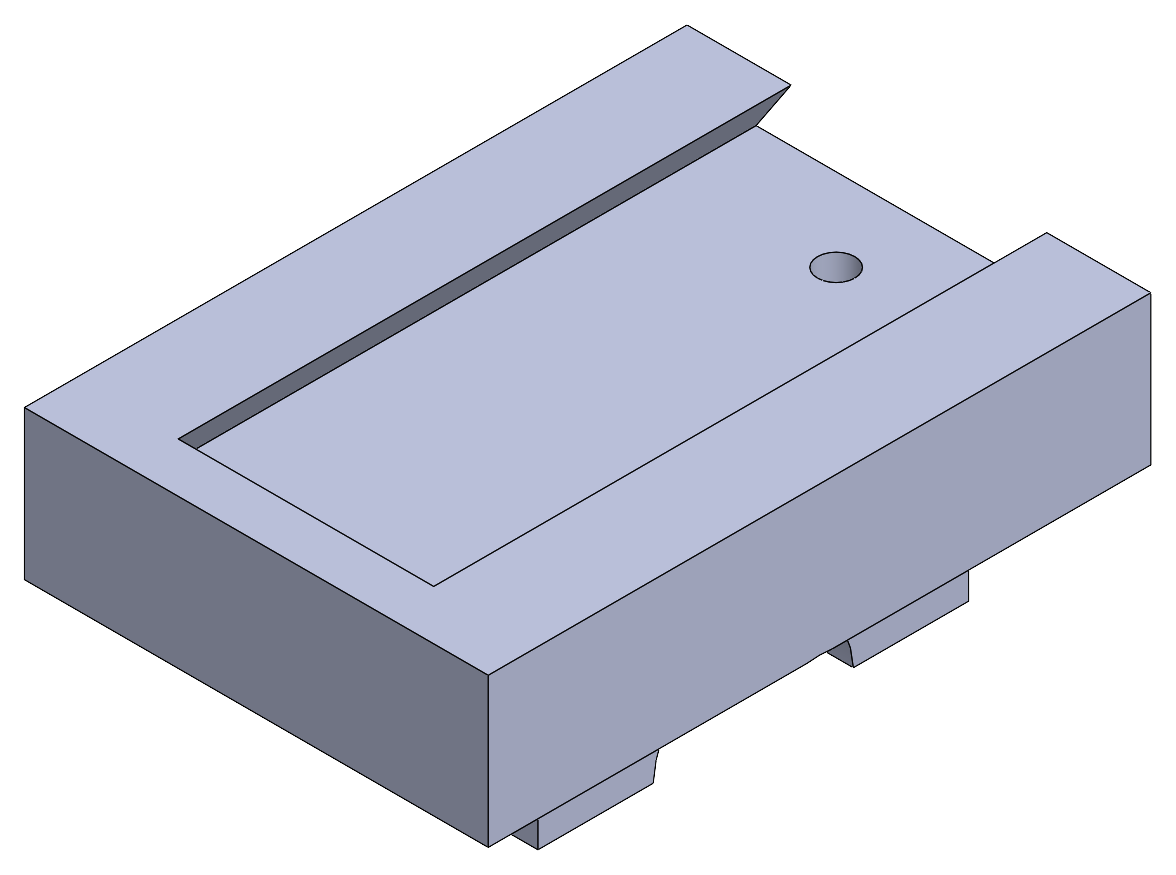
\includegraphics[width=0.31\textwidth]{figures/cad/dash_bracket.png}}
\subfigure[Clamp cap.]{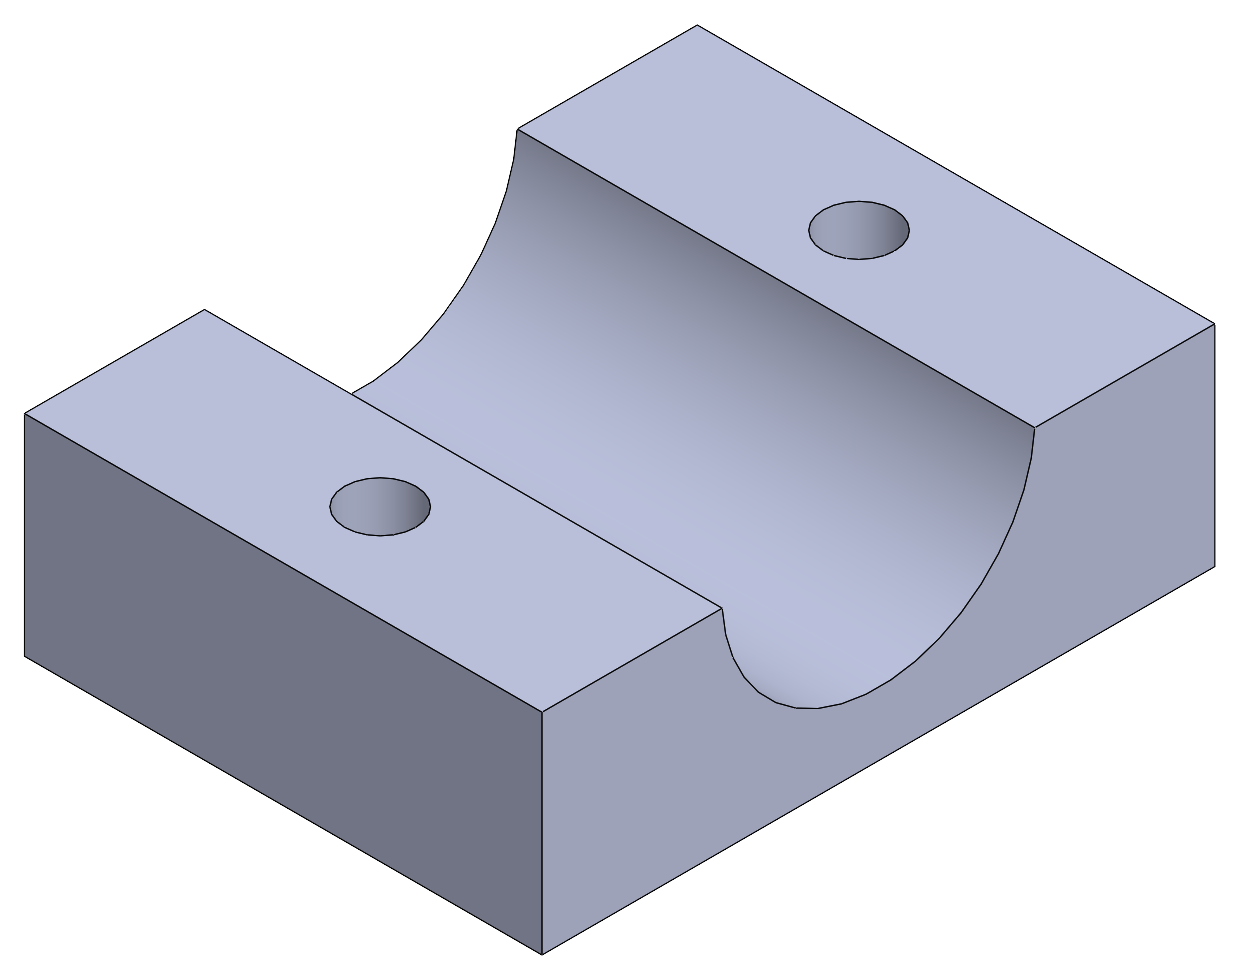
\includegraphics[width=0.31\textwidth]{figures/cad/dash_clamp_cap.png}}
\subfigure[Rail plate with the lock detents.]{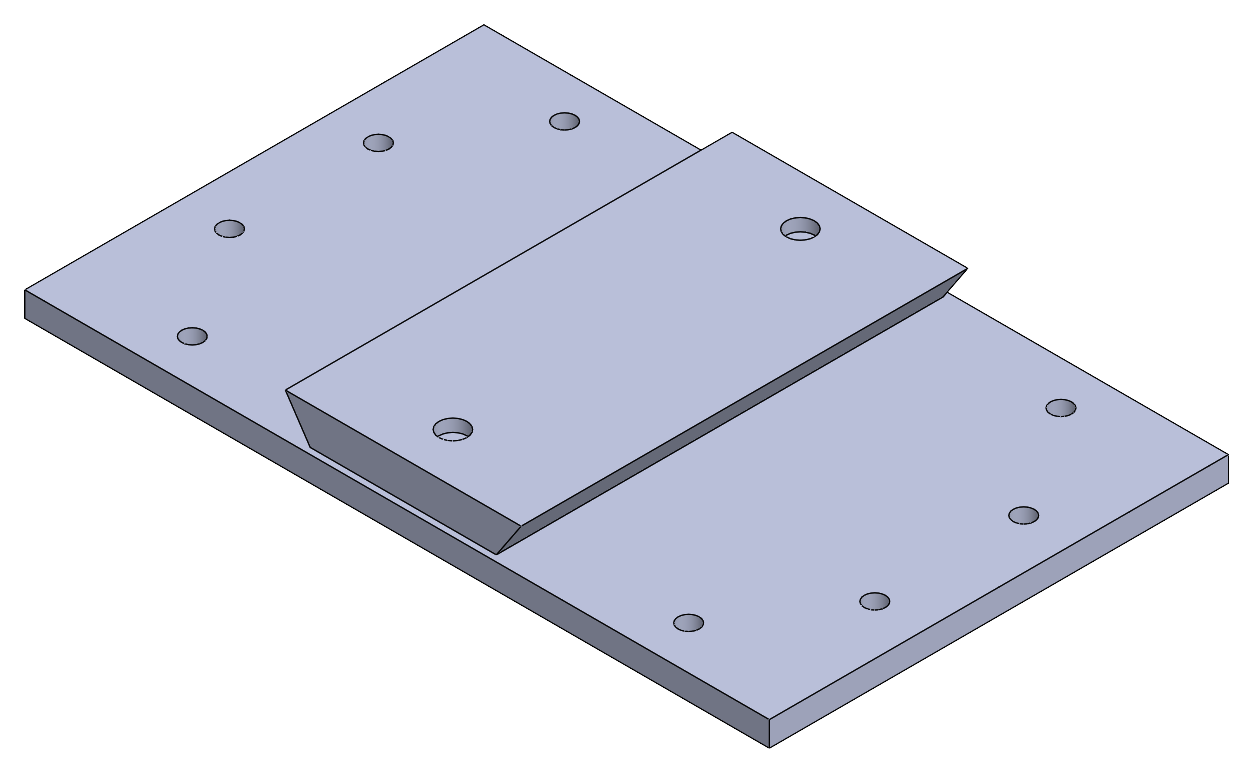
\includegraphics[width=0.31\textwidth]{figures/cad/dash_rail_plate.png}}
\subfigure[Pi~5 cradle with vent slots.]{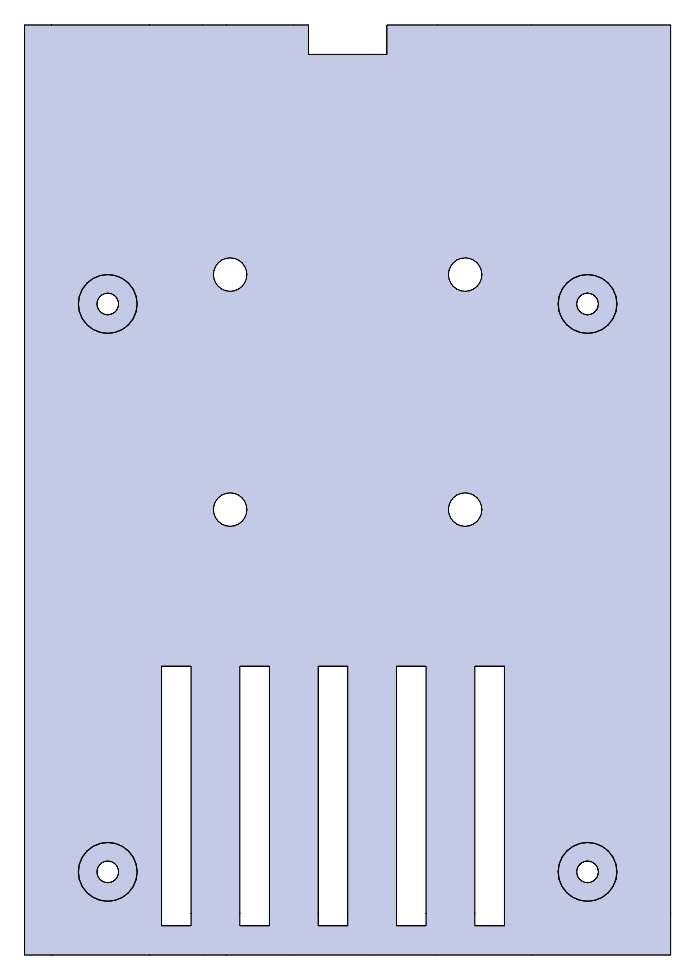
\includegraphics[width=0.25\textwidth]{figures/cad/dash_pi5_cradle.png}}
\subfigure[One of the four shell quarters.]{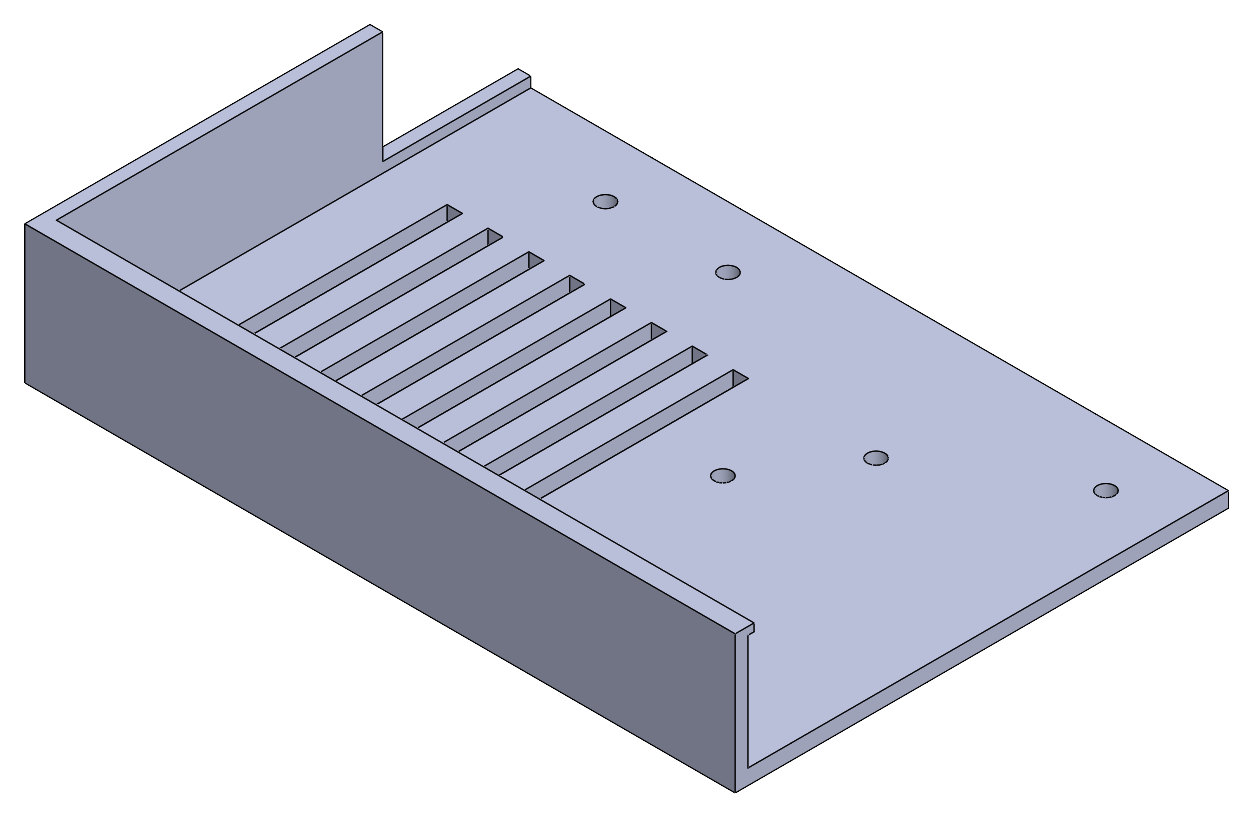
\includegraphics[width=0.4\textwidth]{figures/cad/dash_shell_quarter.png}}
\caption{Printed parts of the dashboard display mount.}
\label{fig:mech-dash-parts}
\end{figure}

\begin{table}[htbp]
\centering
\caption{Dashboard display mount: printed parts.}
\label{tab:mech-dash-parts}
\small
\begin{tabular}{|p{3.4cm}|p{2.6cm}|p{0.7cm}|p{7.2cm}|}
\hline
\textbf{Part} & \textbf{Size (mm)} & \textbf{Qty} & \textbf{Function} \\ \hline
Shell quarter & 139.1 by 96.6 by 27 & 4 & Back shell. The display presses in past 1.2\,mm lips on the long walls \\ \hline
Rail plate & 120 by 74 by 10 & 1 & Dovetail rail (30 to 38\,mm, 72\,mm long, two lock detents); joins the bottom quarters \\ \hline
Cross joiner & 40 by 40 by 3 & 1 & One bolt into each quarter at the centre \\ \hline
Joiner plate & 44 by 20 by 3 & 2 & Across the top and right ends of the joints \\ \hline
Pi~5 cradle & 66 by 95 by 10 & 1 & Holds the Pi~5 on 7\,mm standoffs; joins the left quarters \\ \hline
Bracket & 56 by 80 by 29 & 1 & Dovetail channel (closed end, 0.35\,mm parallel clearance), M4 lock insert, upper clamp half with two 10\,mm M5 inserts \\ \hline
Clamp cap & 40 by 52 by 16 & 1 & Lower clamp half, 4.9\,mm under the bore, 1.5\,mm squeeze gap \\ \hline
\end{tabular}
\end{table}

\section{Rear sensor pod (Raspberry Pi~4 and telemetry unit)}
\label{sec:mech-pod}
It was designed as the front pod before the two-sided layout of 15 October (Section~\ref{sec:two-sided}) and now serves the rear, beside the battery.


The pod (Figures~\ref{fig:mech-pod-assembly} and~\ref{fig:mech-pod-parts}) has a sensor head and an electronics box, bolted together by four M3 flange screws.
\begin{itemize}
\item \emph{Sensor head.} The camera case sits in a cradle above the ToF board, with a foam ring at its front. The three ToF sensors look out through flared windows. The head is an upper shell and a tray that meet at a lip seam.
\item \emph{Electronics box.} The Raspberry Pi~4 and its fan sit in the front bay. The ESP32 board sits in the rear bay, under the thinned roof. A side hatch gives access to the flash drive. There is an SMA bulkhead for the LTE antenna and a gland for the vehicle supply. A sunshade covers the Pi bay.
\item \emph{Mount.} A rail plate under the box takes the same clamp as the display. Its closed end faces forward, so braking pushes the pod against the stop.
\end{itemize}

The two lower flange bolts sit under the Pi~4, so the head must be bolted on before the Pi goes in. The review found this, and the assembly sequence was corrected. Table~\ref{tab:mech-pod-parts} lists the parts.

\begin{figure}[htbp]
\centering
\subfigure[Assembly on the dummy bar.]{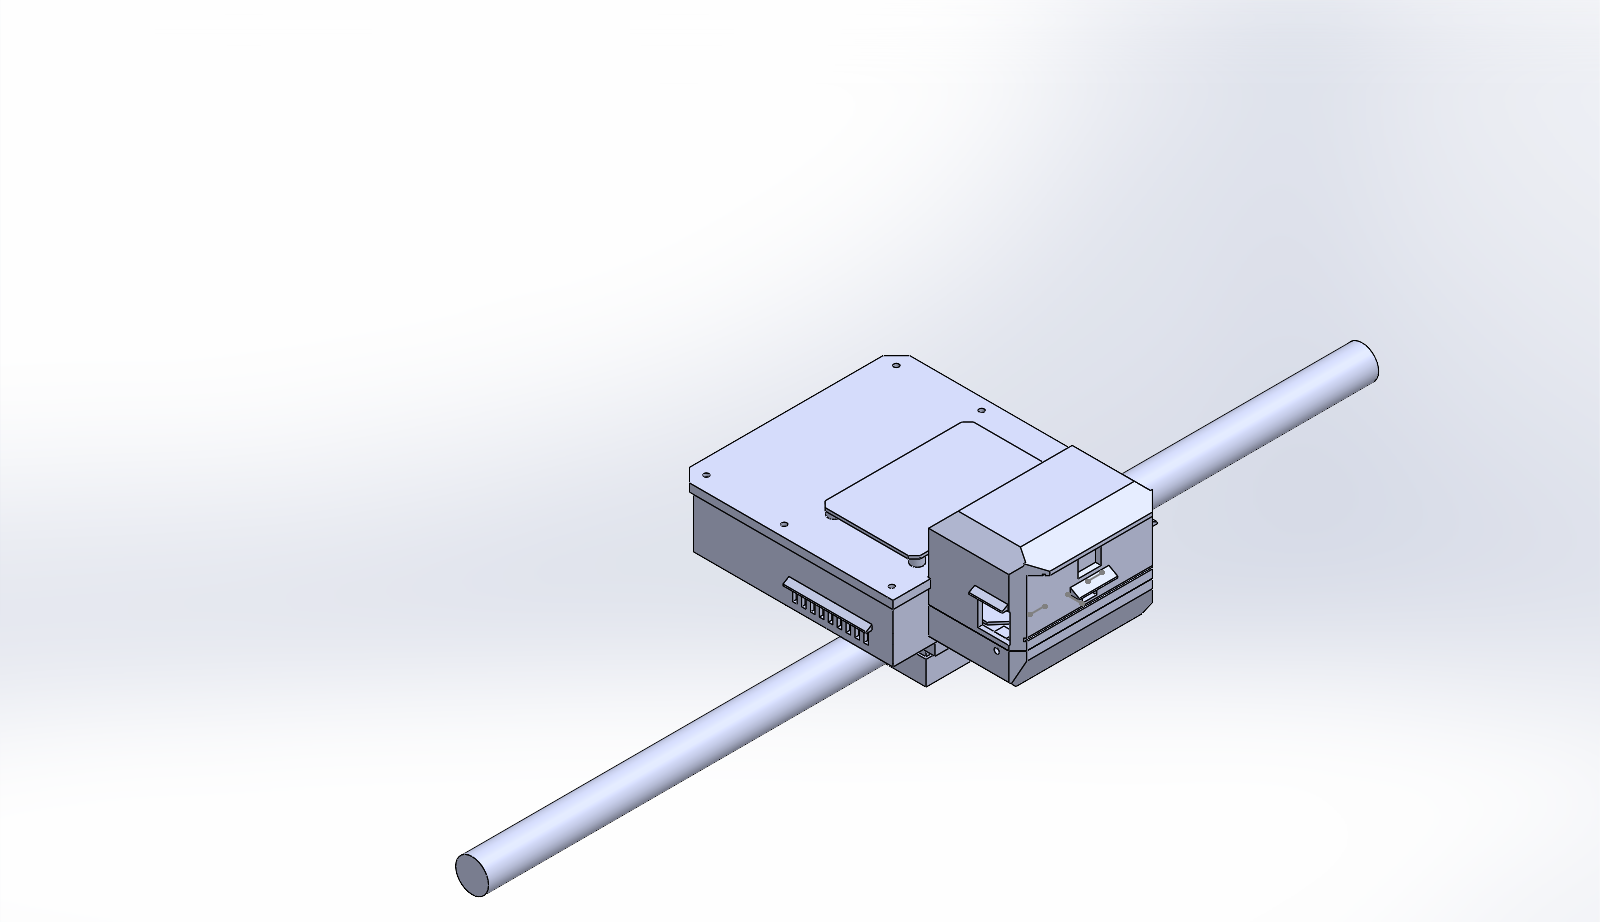
\includegraphics[width=0.48\textwidth]{figures/cad/pod_assembly_iso.png}}
\subfigure[Side view: head (right), box, rail plate and clamp.]{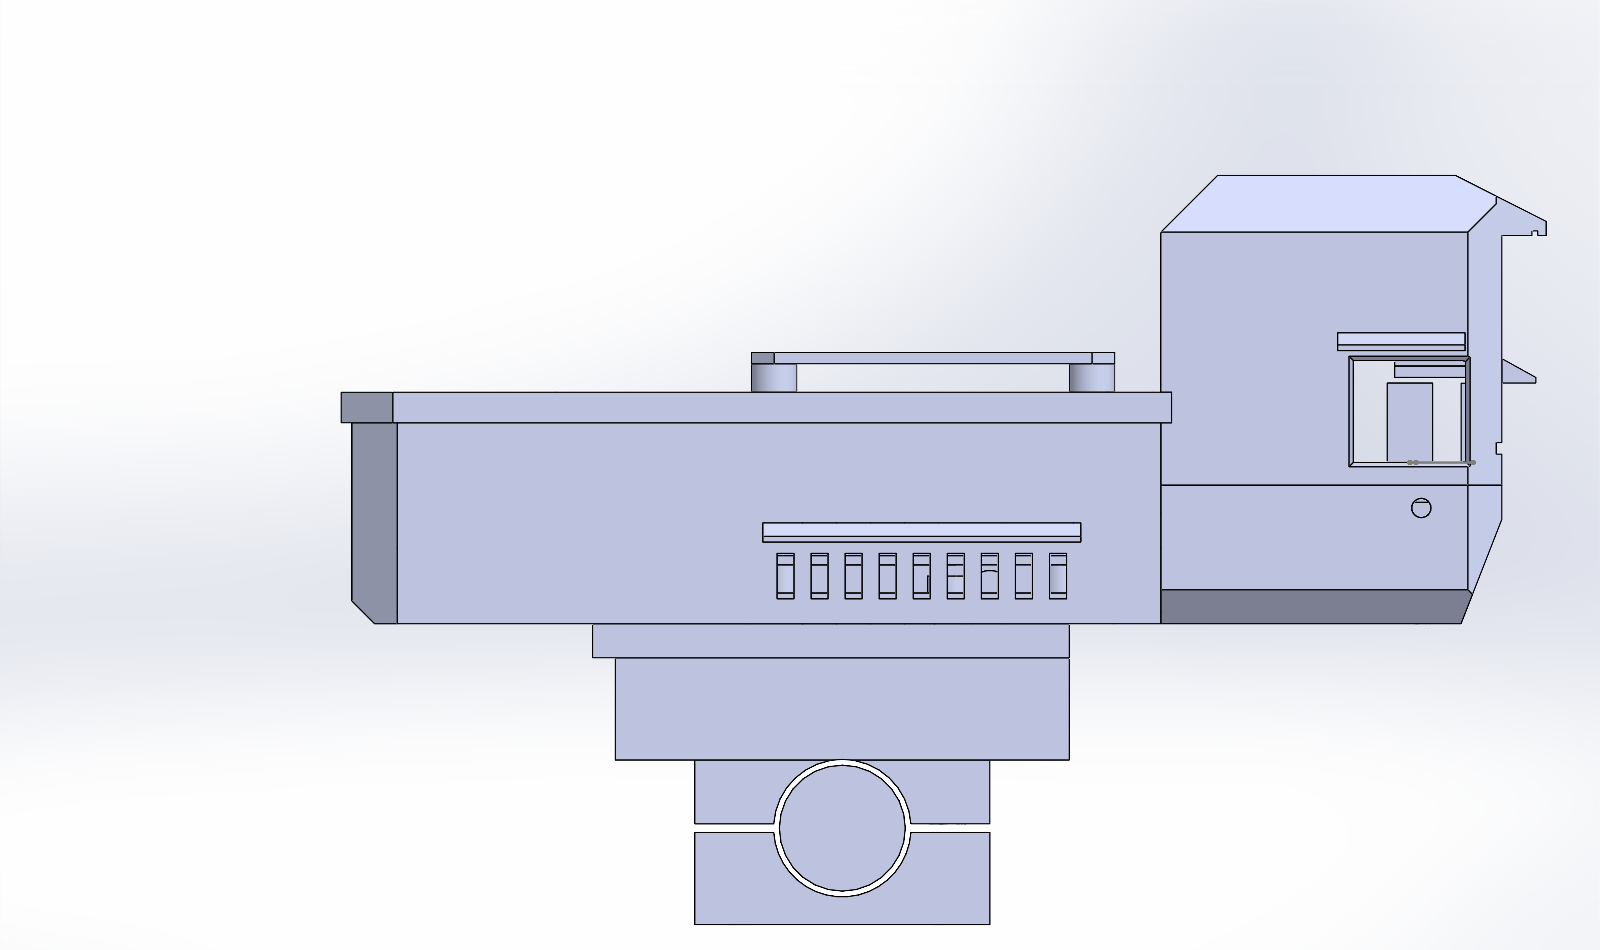
\includegraphics[width=0.48\textwidth]{figures/cad/pod_assembly_side.png}}
\subfigure[From above, with the view cones of the three ToF sensors (25$^\circ$) and the camera (53.5$^\circ$) shown as reference bodies; no cone meets a wall.]{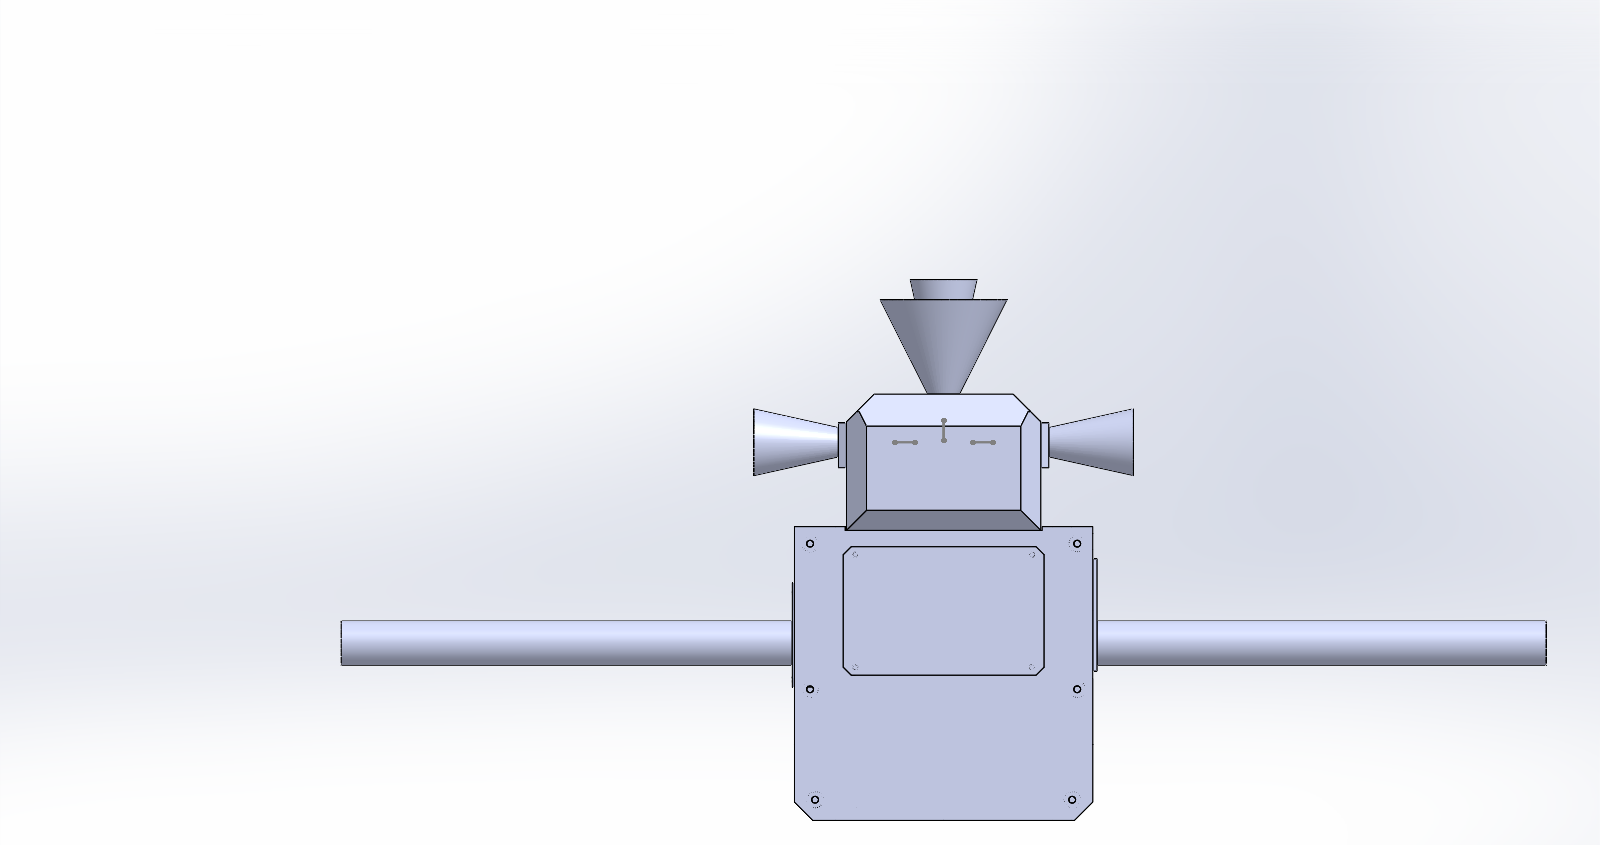
\includegraphics[width=0.6\textwidth]{figures/cad/pod_assembly_cones.png}}
\caption{Rear sensor pod assembly (revision 2).}
\label{fig:mech-pod-assembly}
\end{figure}

\begin{figure}[htbp]
\centering
\subfigure[Head upper shell: brow, windows with hoods, flange bosses.]{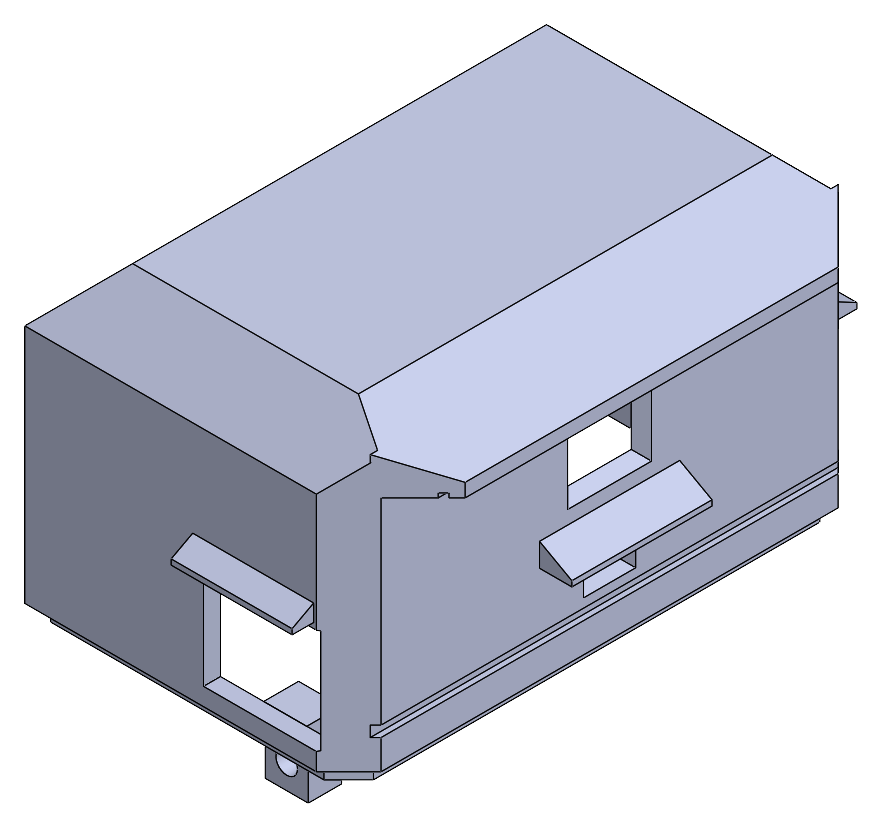
\includegraphics[width=0.31\textwidth]{figures/cad/pod_head_upper.png}}
\subfigure[Head tray: board pillars, ribbon guide, jumper channel.]{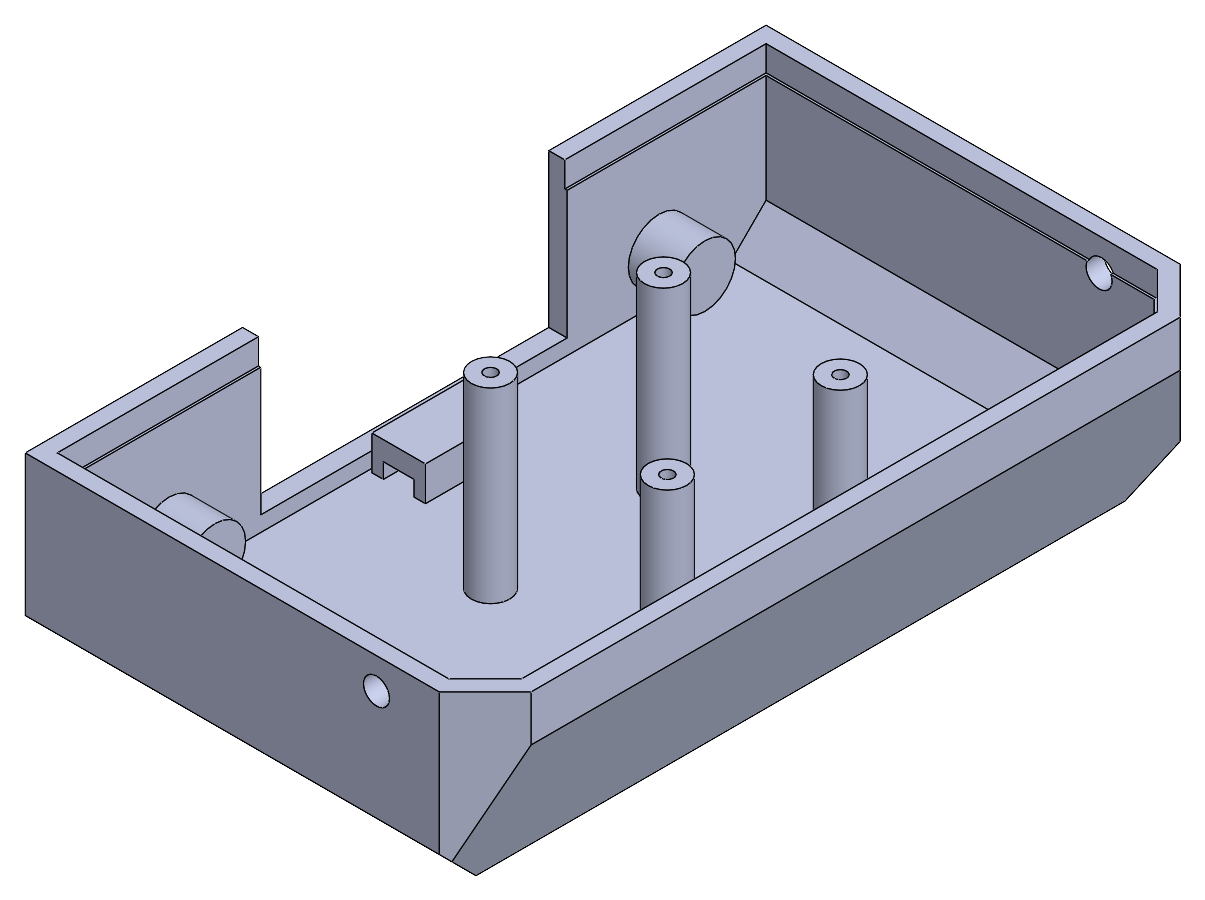
\includegraphics[width=0.31\textwidth]{figures/cad/pod_head_tray.png}}
\subfigure[Electronics box base: Pi~4 and ESP32 bays, vents, hatch.]{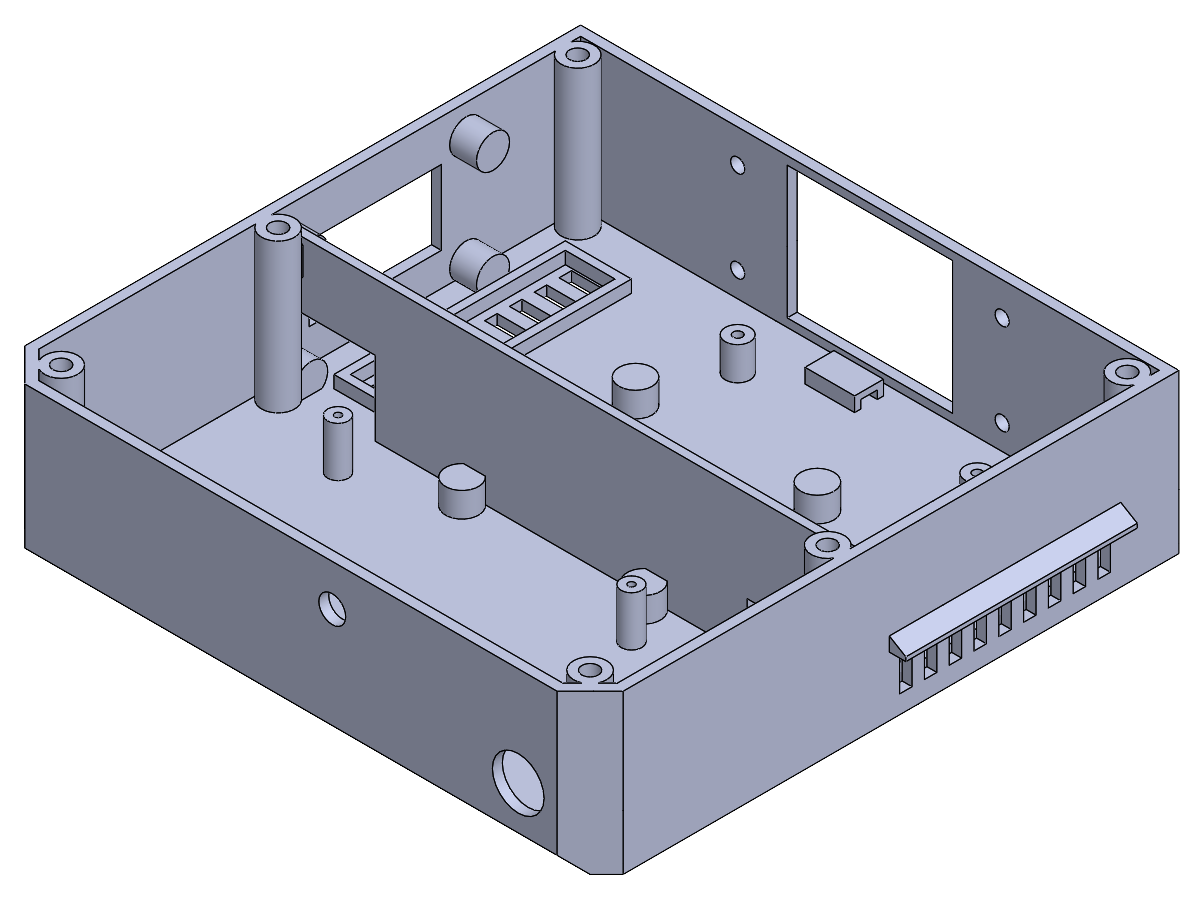
\includegraphics[width=0.31\textwidth]{figures/cad/pod_box_base.png}}
\caption{Main printed parts of the rear sensor pod.}
\label{fig:mech-pod-parts}
\end{figure}

\begin{table}[htbp]
\centering
\caption{Rear sensor pod: printed parts.}
\label{tab:mech-pod-parts}
\small
\begin{tabular}{|p{3.6cm}|p{2.8cm}|p{8.0cm}|}
\hline
\textbf{Part} & \textbf{Size (mm)} & \textbf{Function} \\ \hline
Head upper shell & 104.8 by 67.9 by 63.1 & Camera cradle, ToF windows with drip hoods, brow over the camera, flange bosses \\ \hline
Head tray & 96.8 by 60.1 by 26.8 & Board pillars (estimated hole positions), ribbon guide, jumper channel and tie anchor \\ \hline
Camera retainer & 37.8 by 16.2 by 2 & Holds the camera case in its cradle \\ \hline
Box base & 148.8 by 142.5 by 38.4 & Pi~4 and ESP32 standoffs, 5\,V converter space, vents with hoods, hatch, gland, SMA hole, insert bosses \\ \hline
Box lid & 148.6 by 146.3 by 5.4 & Tongue-and-skirt seam, thinned roof over the GNSS patch \\ \hline
Sunshade & 100 by 64 by 7 & Second roof over the Pi bay, on four posts \\ \hline
USB hatch cover & 52 by 33.5 by 5.4 & Closes the side hatch \\ \hline
Rail plate & 84 by 60 by 12 & Dovetail rail with lock detents \\ \hline
\end{tabular}
\end{table}

\section{IMU pods}
\label{sec:mech-imu}

Each IMU pod holds one GY-521 board. The pods printed and fitted are revision 3 (Figures~\ref{fig:mech-imu} and~\ref{fig:mech-imu3}). An engraved arrow on the lid marks the vehicle's forward direction, and cable ties through the ears fix the pod to the stem or the chassis rail. On the road session of 19 October both pods were at the rear, side by side on the chassis next to the telemetry unit, so the two IMUs measured the same motion. From 22 October one IMU moved to the front node, so each end of the vehicle has its own (Section~\ref{sec:firmware}).

\begin{figure}[htbp]
\centering
\subfigure[Base: ledges, pegs, connector bay with wire slot, four cable-tie ears.]{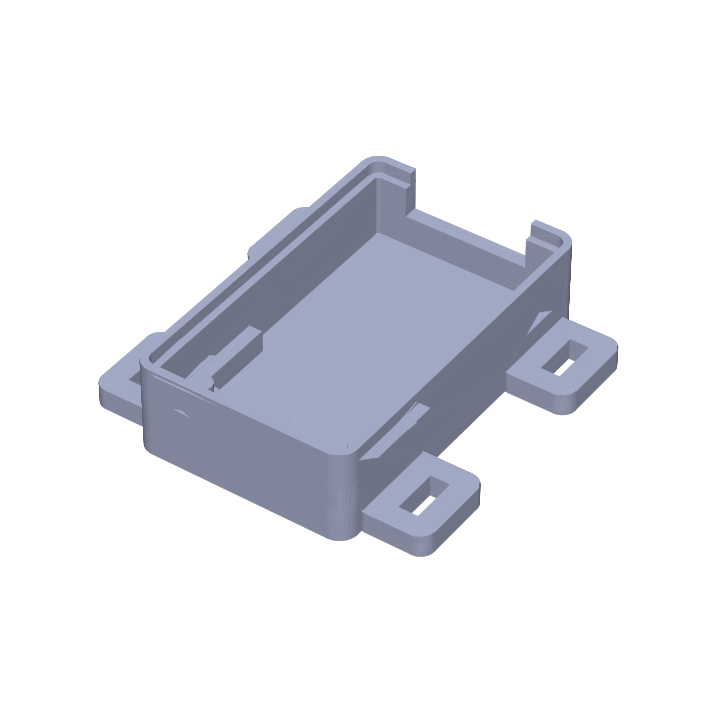
\includegraphics[width=0.44\textwidth]{figures/cad/imu_pod_rev3_base.png}}
\subfigure[Lid, underside: half-lap rim and the two tubes that press the board onto the pegs.]{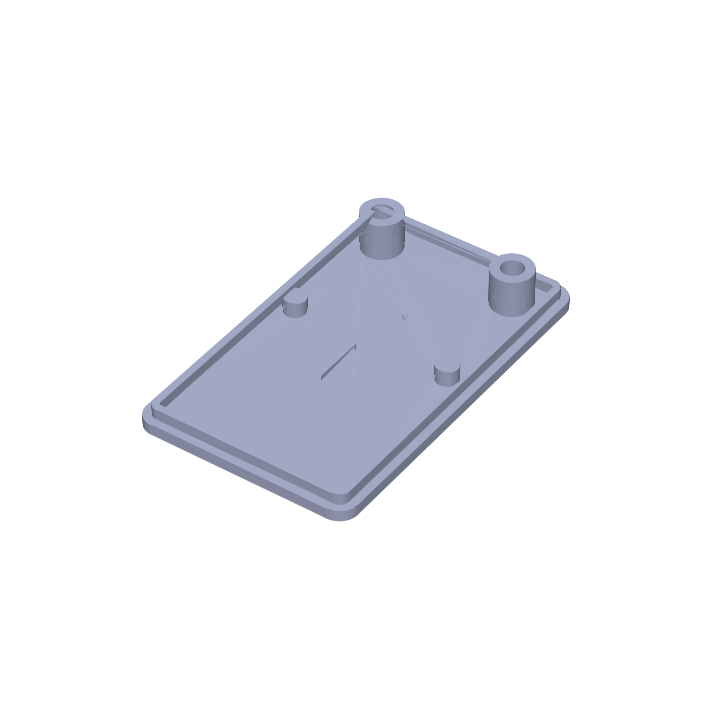
\includegraphics[width=0.44\textwidth]{figures/cad/imu_pod_rev3_lid.png}}
\caption{IMU pod (revision 3, as printed and fitted), rendered from the printed STL files.}
\label{fig:mech-imu}
\end{figure}

Revision 2 was a solid block with a pocket of 0.6\,mm clearance, the board screwed down on its hole edge and held at the free edge by a lid rib and foam pad, with the wires soldered to the pads. The first printed pod showed two faults in a fit test: the boards carry a right-angle header whose Dupont housings stand out past the board edge, so the lid could not close, and no screws were to hand. Revision 3 (13 October) follows the push-fit style of the camera case:
\begin{itemize}
\item 1.6\,mm walls instead of a solid block; 24 by 39 by 11.6\,mm with the lid;
\item the board on ledges 2.5\,mm above the floor, clear of the header's solder tails, located by two pegs in its holes;
\item clearance reduced to 0.4\,mm a side at the student's request;
\item tubes under the lid press the board onto the pegs, so no screws are used;
\item the lid pushes onto a half-lap rim with a 0.1\,mm gap;
\item an 18\,mm bay for the Dupont housings, with a wire slot closed by the lid;
\item four cable-tie ears.
\end{itemize}
Two pods print in 1\,h 19\,min from 13.7\,g, against 2\,h 28\,min for revision 2. The geometry is scripted (\texttt{CAD/\allowbreak{}IMU\_\allowbreak{}Pod/\allowbreak{}rev3/\allowbreak{}imu\_\allowbreak{}pod\_\allowbreak{}rev3.py}), and the script checks that lid and base do not overlap. The peg spacing uses the unmeasured 15.2\,mm hole spacing, with about 1\,mm of play.

\begin{figure}[htbp]
\centering
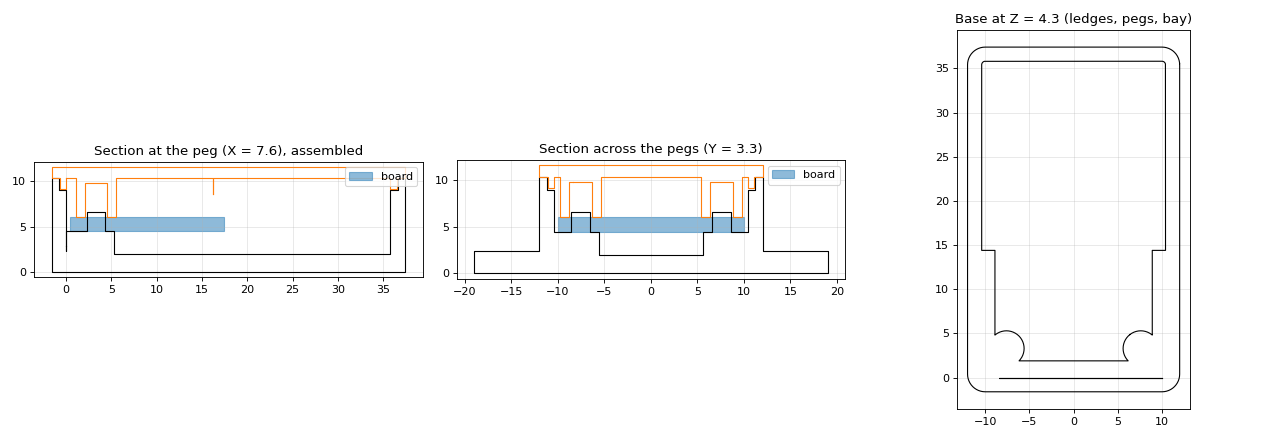
\includegraphics[width=\textwidth]{figures/cad/imu_pod_rev3_sections.png}
\caption{IMU pod revision 3, sections: board (blue) on its ledges and pegs, lid (orange) with the tubes over the pegs, connector bay to the right.}
\label{fig:mech-imu3}
\end{figure}

\section{Front sensor pod for the Raspberry Pi~5}
\label{sec:mech-fpod}

The two-sided layout (Section~\ref{sec:two-sided}) needs a second sensor pod at the front for the Raspberry Pi~5, which carries the AI HAT+ (Hailo accelerator) on its own cooler. It keeps the original head (camera, time-of-flight board, windows and hoods) on a new box for the computer alone (\texttt{CAD/Sensor\_Pod\_Front}; Figure~\ref{fig:mech-fpod}).

\begin{itemize}
\item \emph{Reused parts.} An identity audit compared volume, area, centre of mass, bounding box and face count. The head tray, camera retainer and rail plate match the original parts, and the head upper matches the sliced original once a drip lip that the original script adds, but the saved part lacks, is left out. So beds 08, 09 and 12 serve both pods.
\item \emph{The stack.} The box was raised by 16\,mm to 153 by 117 by 56\,mm. It holds, from the bottom: the Raspberry Pi~5 on 10\,mm standoffs; the official cooler; the AI HAT+ on 16\,mm spacers; and the Hailo with an assumed 8\,mm heatsink. The time-of-flight jumpers plug onto the stacking pins above the HAT, and the camera ribbon drops through the HAT's slot (164\,mm path, leaving 36\,mm of the 200\,mm cable).
\item \emph{Cooling.} The cooler blows out through low slots in one wall; slots higher in both side walls give air across the HAT and the Hailo. The lid has an exhaust grille under a hood (below).
\item \emph{Fixing.} M2.5 by 16 screws from under the floor through the standoffs into the HAT's spacers. A 22\,mm gap lets a hex key reach the head's lower flange bolts with the computer fitted, which removes an assembly-order problem of the original pod.
\end{itemize}

The six audit findings were fixed: thin insert walls, a 0.32\,mm skin under the screw heads, two slivers, a short insert cap, thin drip-ledge tips and bosses that would print in mid-air. The assembly then measured:
\begin{itemize}
\item no interference;
\item every fastener hole coaxial;
\item every insert wall at least 2.0\,mm;
\item the Hailo's heatsink 14.8\,mm from the lid, and the jumper loop 3.3\,mm from it;
\item the hex keys clear of everything by 2.7\,mm.
\end{itemize}
A last change, moving two bosses that came within 0.28\,mm of a USB plug, was not re-audited, because the CAD program crashed twice during the full-assembly check. The spacer height, the heatsink and the cable length are datasheet values or estimates to be measured. The new parts print in about 20 hours from 250\,g of PLA: the box base without supports, the lid and hood, and one bed of rail plate, sunshade and port covers.

\begin{figure}[htbp]
\centering
\subfigure[Assembly on a dummy bar: head, box and lid.]{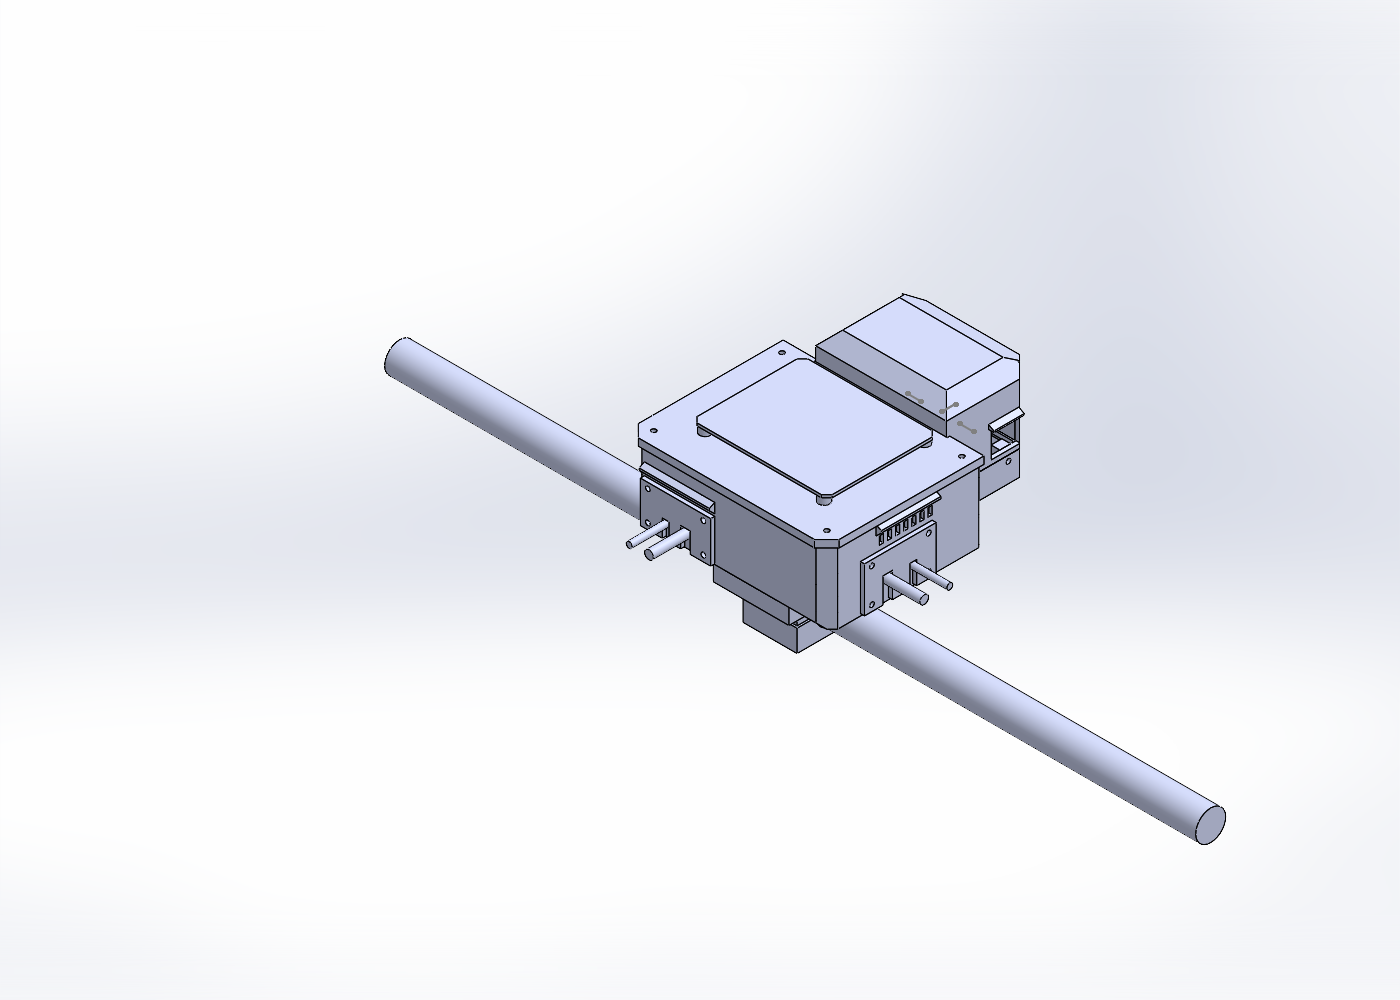
\includegraphics[width=0.48\textwidth]{figures/cad/fpod_assembly_iso.png}}
\subfigure[Side view with the walls hidden: computer, cooler, AI HAT+, Hailo heatsink, jumper loop and camera ribbon.]{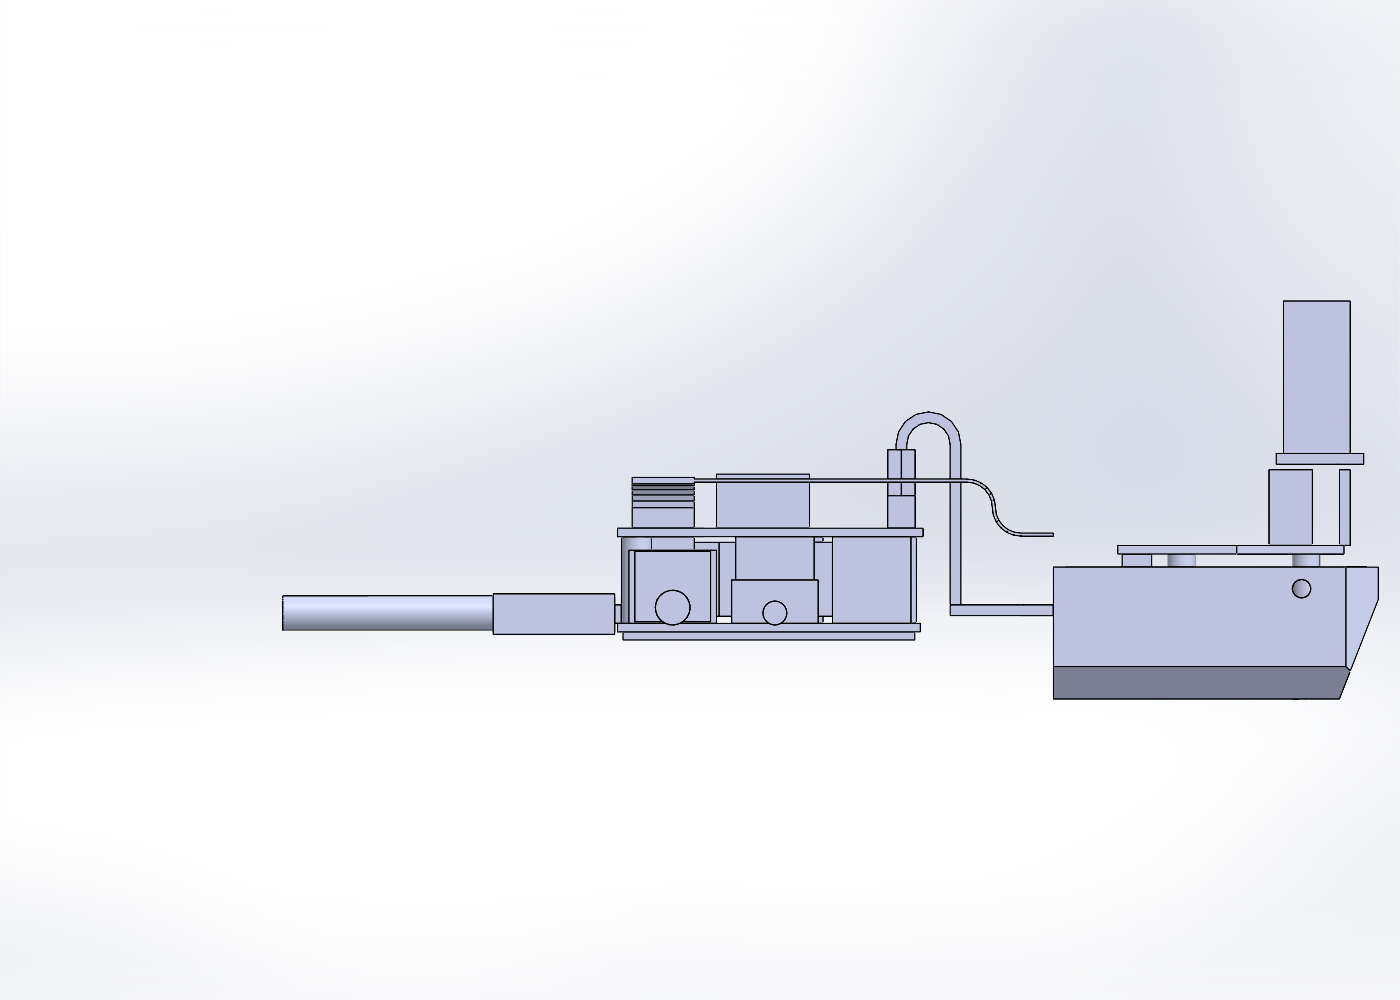
\includegraphics[width=0.48\textwidth]{figures/cad/fpod_internals_side.png}}
\subfigure[Box base and vented lid, rendered from the print files.]{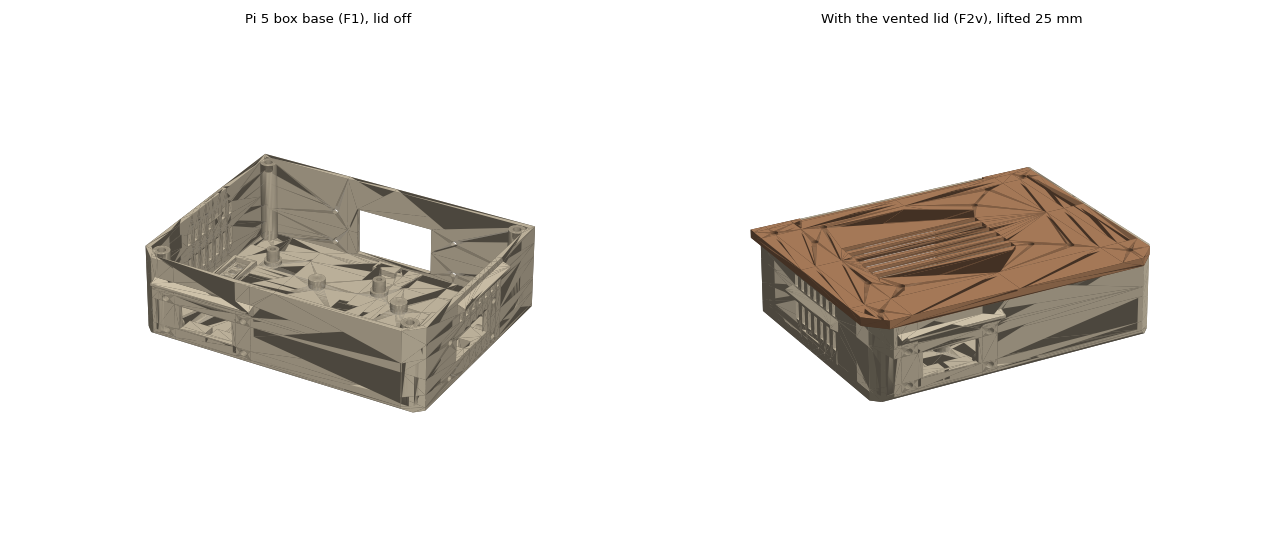
\includegraphics[width=0.7\textwidth]{figures/cad/fpod_box_render.png}}
\caption{Front sensor pod for the Raspberry Pi~5 and AI HAT+.}
\label{fig:mech-fpod}
\end{figure}

\section{Ventilated lids}
\label{sec:mech-vent}

In the closed rear box the Raspberry Pi~4 reached 76.9\,\textdegree C (Section~\ref{sec:inv-power}): the box's only vents were in the floor and low in one wall, and nothing let warm air out at the top. Both pods' lids now have an exhaust grille over the computer, seven 4\,mm slots giving about 1,900\,mm$^2$ open. A separate hood stands 10\,mm above the grille, closed at the front and sides and open to the rear with a drip lip, so warm air leaves and rain and the head wind stay out (Figure~\ref{fig:mech-vent}).

Four pins on the hood push into holes in the lid, so no screws are needed. Both parts print flat without supports: the rear lid in 3\,h 39\,min, the front lid in 3\,h 00\,min, and each hood in about 1\,h 25\,min. The lids were changed from the exported parts with a script (\texttt{CAD/\allowbreak{}Sensor\_\allowbreak{}Pod/\allowbreak{}vent\_\allowbreak{}rev/\allowbreak{}lid\_\allowbreak{}vent.py}), which checks that hood and lid do not overlap. The temperature in the vented boxes has not yet been measured.

\begin{figure}[htbp]
\centering
\subfigure[Rear pod (Raspberry Pi~4 and telemetry unit).]{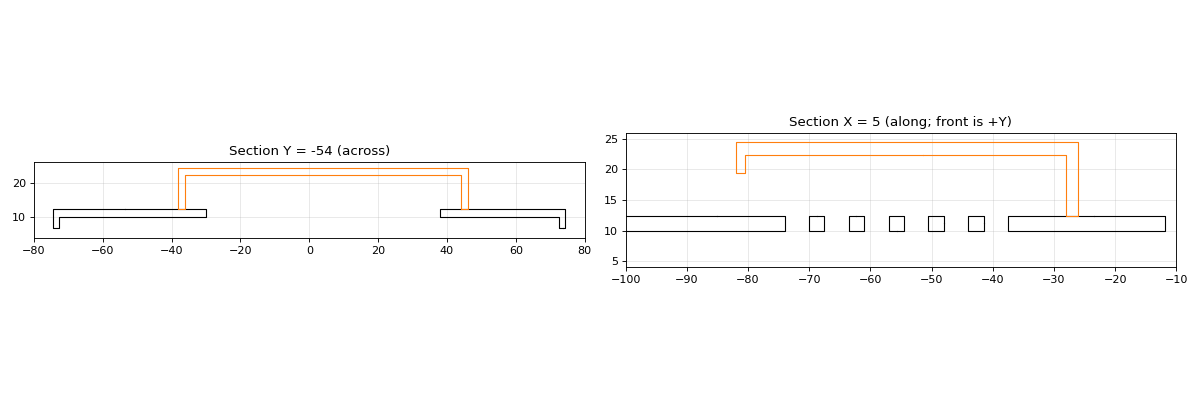
\includegraphics[width=\textwidth]{figures/cad/lid_vent_sections.png}}
\subfigure[Front pod (Raspberry Pi~5 and AI HAT+).]{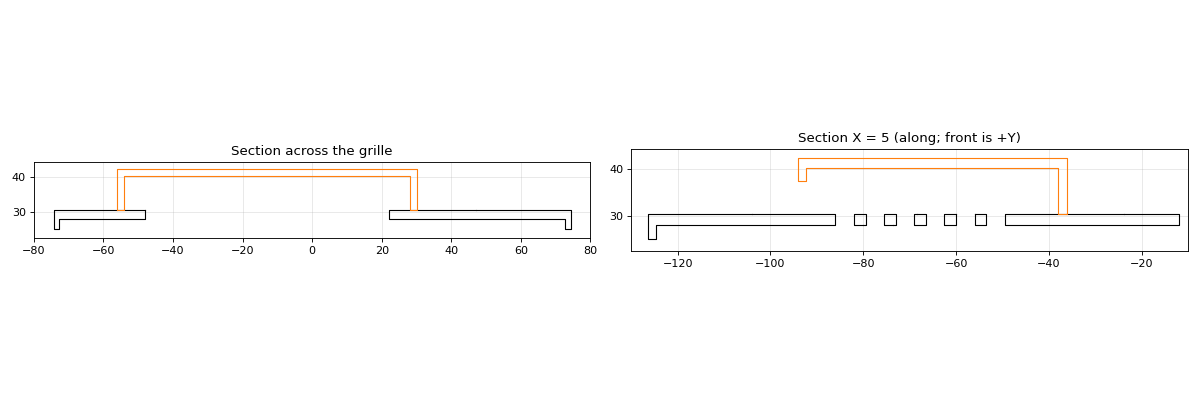
\includegraphics[width=\textwidth]{figures/cad/fpod_lid_vent_sections.png}}
\caption{Ventilated lids, sections: lid (black) with the grille, hood (orange) open to the rear.}
\label{fig:mech-vent}
\end{figure}

\section{Verification of the geometry}
\label{sec:mech-verification}

Each design was audited in its saved SOLIDWORKS files by scripts (\texttt{CAD/*/build/audit\_*.py}). The scripts read the actual three-dimensional geometry, not a rendering, and their results are in each design's \texttt{ENGINEERING\_REVIEW.md}. Five checks were run:
\begin{itemize}
\item \emph{Interference.} SOLIDWORKS interference detection over the whole assembly. Before each result was trusted, a deliberately overlapping probe part was added to prove the check reports overlaps.
\item \emph{Contacts.} Every part must touch the parts it fastens to, so that nothing floats.
\item \emph{Fasteners.} Every screw position must have a hole of the right size in both parts, coaxial within 0.05\,mm.
\item \emph{Thin walls.} Every pair of opposing faces closer than 2\,mm.
\item \emph{Parts.} Body count, geometry faults and fit on the print bed.
\end{itemize}

The first review of the display mount rejected it. Its three critical defects:
\begin{itemize}
\item the clamp cap's bore cut right through it, leaving two loose pieces;
\item the M5 inserts had 0.2\,mm of wall;
\item the shell's bolt holes were mirrored, so the rail plate's holes did not line up.
\end{itemize}

It also had five major defects:
\begin{itemize}
\item the cross joiner and rail plate overlapped by 1146\,mm\textsuperscript{3};
\item the side lock screw's head would hit the rail plate;
\item the clamp had no squeeze gap;
\item there was no room for nuts behind the display;
\item the dovetail flanks were not parallel.
\end{itemize}

The mirrored holes came from a sign error between the sketch plane's axes and the model's. All were corrected in the scripts and the parts rebuilt (revision 2). The audits were then run again; Table~\ref{tab:mech-verification} gives the results. Two corrections first introduced new thin walls of 1.0 and 1.75\,mm, which the wall audit caught before the parts were saved. The IMU pod column is for revision 2; revision 3, which was printed, has no screws, and its own script checks only that lid and base do not overlap (Section~\ref{sec:mech-imu}).

\begin{table}[htbp]
\centering
\caption{Geometry checks after revision 2 (12 October).}
\label{tab:mech-verification}
\small
\begin{tabular}{|p{3.0cm}|p{3.8cm}|p{3.8cm}|p{3.8cm}|}
\hline
\textbf{Check} & \textbf{Display mount} & \textbf{Sensor pod} & \textbf{IMU pod (revision 2)} \\ \hline
Probe overlap detected & Yes (1564\,mm\textsuperscript{3}) & Yes (79\,057\,mm\textsuperscript{3}) & Yes (1303\,mm\textsuperscript{3}) \\ \hline
Hard interference & 0 & 0, including the view cones & 0 \\ \hline
Fastener holes & All matched (16 shell bolts, M5 clamp) & All 30 joints and 12 board pilots & All 4 lid screws \\ \hline
Walls under 2\,mm & Pi~5 standoffs 1.9\,mm (minor); lips 1.5\,mm (by design) & None in the printed load paths & 1.35\,mm, pilot bottom to strap tunnel, below the screw's reach \\ \hline
Dovetail clearance & 0.350\,mm on both flanks, parallel & Same rail and clamp & Not applicable \\ \hline
Components fixed in assembly & 11 of 11 & 16 of 16 & Not applicable \\ \hline
Fits the 180\,mm bed & All printed parts & All printed parts & Yes \\ \hline
Acceptance & Prototype-ready for the clamp, rail plate and a dovetail coupon & Requires revision (measurements) & Prototype-ready \\ \hline
\end{tabular}
\end{table}

No finite-element analysis was done, because there is no defined load case. The validation route is physical, in four tests:
\begin{itemize}
\item a printed dovetail coupon to check the slide fit;
\item a clamp slip test with 1.5\,kg hung at 150\,mm from the bar;
\item an insert pull-out test;
\item a short ride with a safety tie, checking the bolt torques afterwards.
\end{itemize}

\section{Manufacture}
\label{sec:mech-print}

All parts were sliced with PrusaSlicer 2.9.4 for the Prusa MINI at 0.20\,mm layers, onto 13 beds (Figure~\ref{fig:mech-beds}, Table~\ref{tab:mech-print}).
\begin{itemize}
\item \emph{Load-bearing parts} (clamp, cap and rail plates): 5 perimeters and 50\% infill.
\item \emph{Enclosures}: 3 perimeters and 25\% infill.
\item \emph{Supports}: only under the clamp's half bore, the pod's brow and inside the pod tray and box.
\item \emph{Orientation}: each part is printed with its largest flat face on the bed and the load-bearing layers across the load, as each review specifies.
\end{itemize}

The first prints are in PLA, for checking fits. PLA softens at about 55\,$^\circ$C, so the parts that stay on the vehicle are to be reprinted in PETG or ASA. Two faults in the slicer's command line had to be worked round:
\begin{itemize}
\item two multi-extruder settings in the saved print profile crash it;
\item its \texttt{--merge} option crashes it, even with default settings.
\end{itemize}

For the second, each bed is laid out by the slicing script and sliced as one model, and the script checks that every part is on the bed.

\begin{table}[htbp]
\centering
\caption{Print plan (Prusa MINI, PLA, 0.20\,mm).}
\label{tab:mech-print}
\small
\begin{tabular}{|p{6.0cm}|p{1.0cm}|p{2.6cm}|p{2.2cm}|}
\hline
\textbf{Bed} & \textbf{Prints} & \textbf{Time each} & \textbf{PLA each} \\ \hline
Display shell quarters (4 beds) & 1 each & 3\,h 47\,min to 3\,h 51\,min & 51 to 55\,g \\ \hline
Display rail plate and joiner plates & 1 & 4\,h 22\,min & 51\,g \\ \hline
Pi~5 cradle and cross joiner & 1 & 1\,h 54\,min & 23\,g \\ \hline
Clamp bracket and cap & 2 & 9\,h 0\,min & 95\,g \\ \hline
Pod head upper shell & 1 & 10\,h 18\,min & 114\,g \\ \hline
Pod tray and camera retainer & 1 & 3\,h 2\,min & 35\,g \\ \hline
Pod box base & 1 & 11\,h 23\,min & 130\,g \\ \hline
Pod lid & 1 & 3\,h 42\,min & 56\,g \\ \hline
Pod rail plate, sunshade and hatch cover & 1 & 5\,h 12\,min & 61\,g \\ \hline
Two IMU pods (revision 3) & 1 & 1\,h 19\,min & 13.7\,g \\ \hline
\textbf{Total} & & \textbf{about 74.5\,h} & \textbf{about 0.9\,kg} \\ \hline
\end{tabular}
\end{table}

\begin{figure}[htbp]
\centering
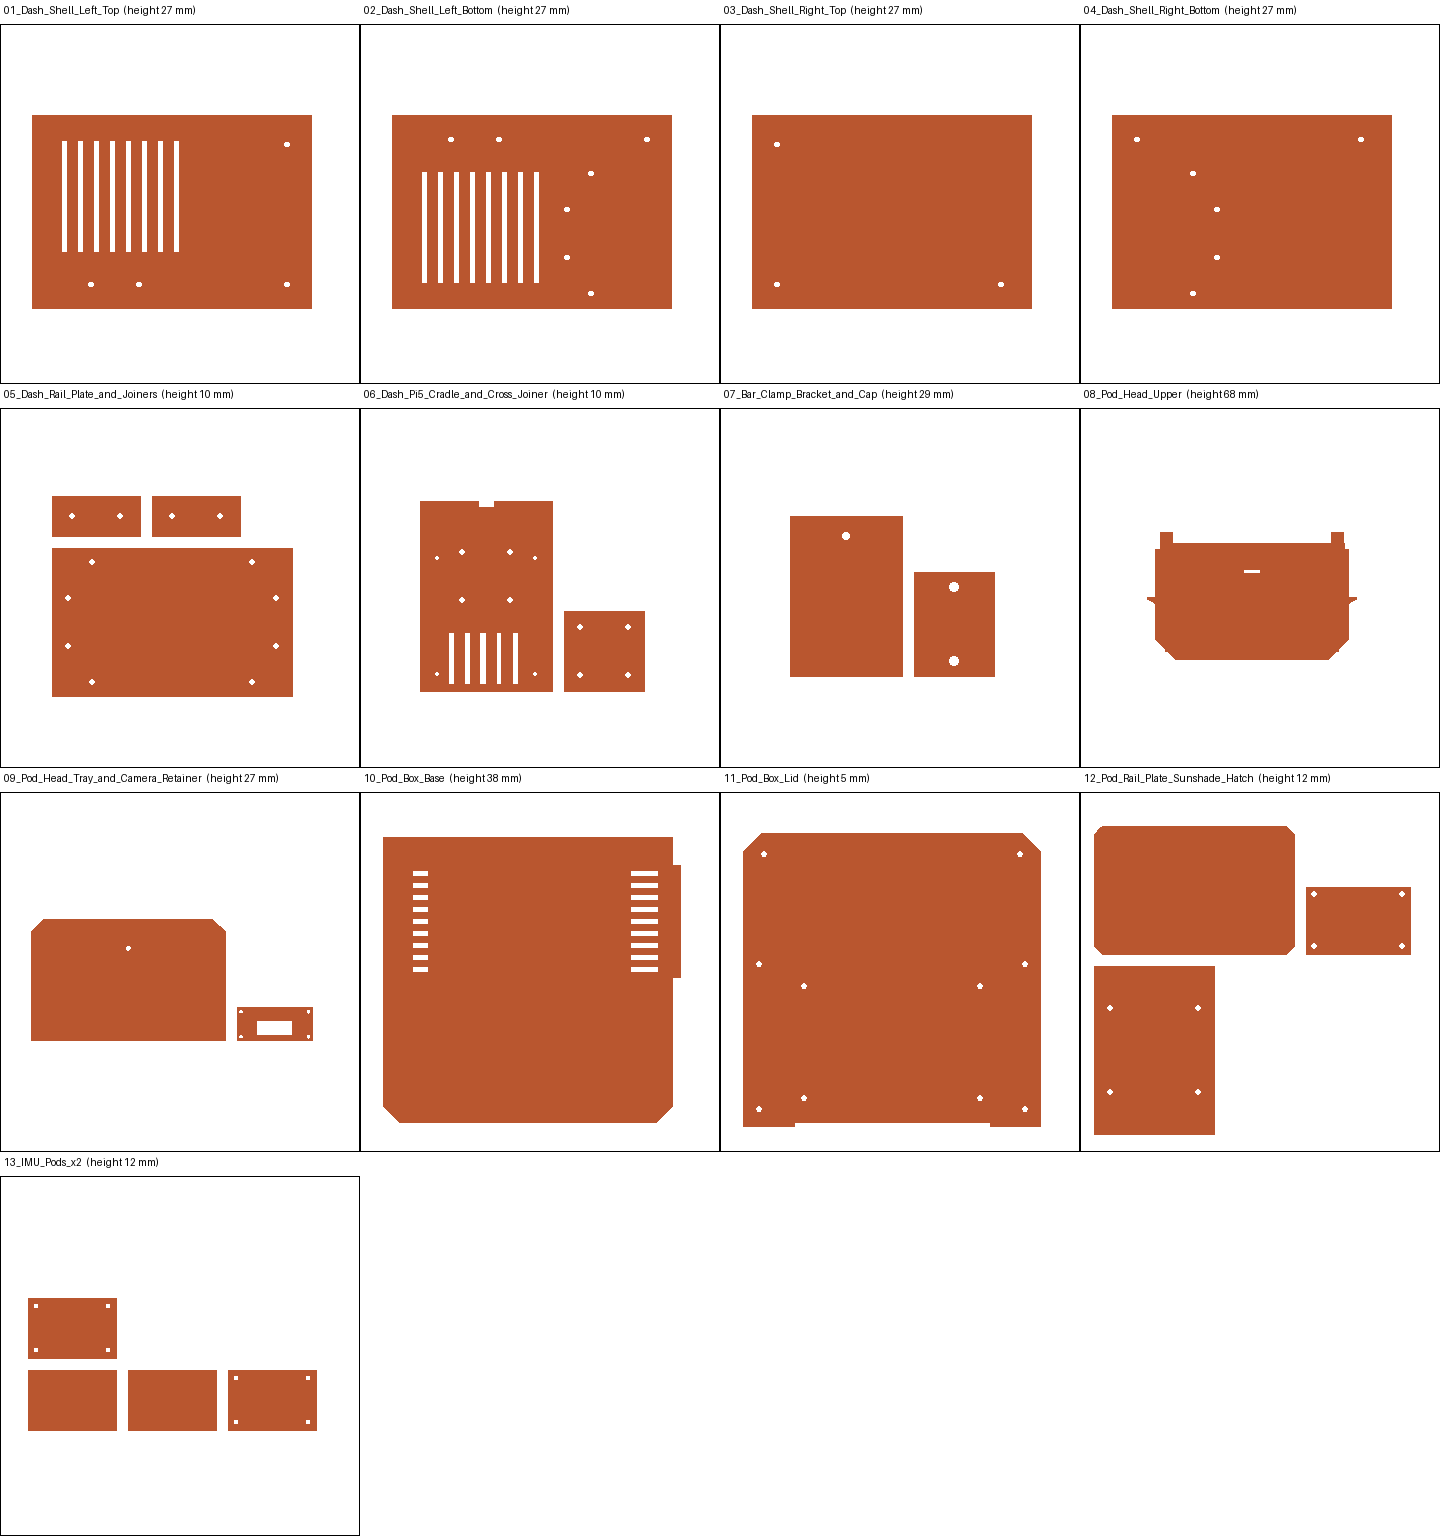
\includegraphics[width=0.85\textwidth]{figures/cad/print_bed_layouts.png}
\caption{Top views of the 13 print beds, drawn from the sliced STL data to check that every part is present and none overlaps.}
\label{fig:mech-beds}
\end{figure}

\section{Status and limitations}
\label{sec:mech-outstanding}

The sensor pods and IMU pods were printed and fitted to the vehicle for the road session of 19 October. Their retention after driving has not been checked against marks, and the physical tests of Section~\ref{sec:mech-verification} have not been run. The dovetail coupon, the bar clamp and the display shell were not printed; they are not needed for the measurements of this report and are future work (Chapter~\ref{chap:recs}).

Several inputs remain estimates and were not measured with calipers: the display's long side, the bar diameter at the clamp, the ToF board's hole positions, the IMU board's hole spacing, the camera ribbon length, the ESP32 battery and GNSS patch sizes, and the 5\,V converter. The parts that were fitted were made to these values.

The side ToF sensors face 90$^\circ$ to each side as built. The fusion configuration, which earlier assumed 35$^\circ$, was set to $\pm 90^\circ$ on 15 October to match the boards, so the pod and the configuration agree; the bearings have not been measured on the mounted pods (test C9).
